\clearpage
\appendix

\section*{Supporting Materials (Not Intended for Print)}

\par This is the Online Appendix of ``Local Bandwagoning and National Balancing: How Uninformed Voters Respond to Partisan Environments and Why It Matters.'' 

\section{Study 1 Appendix} \label{appA}
\setcounter{table}{0}
\renewcommand{\thetable}{A\arabic{table}}
\setcounter{figure}{0}
\renewcommand{\thefigure}{A\arabic{figure}}

\subsection{Variable Constructs} 

\par Knowledge variables in CCES datasets are constructed by aggregating correct answers from following eight questions. The final score is normalized to the 0-1 range: 0 indicates all incorrect, and 1 indicates all correct.

\begin{itemize}
    \item Majority party in the federal House (2008: \textit{CC308a}; 2016: \textit{CC16\_321a})
    \item Majority party in the federal Senate (2008: \texttt{CC308b}; 2016: \texttt{CC16\_321b})
    \item Majority party in the state Senate (2008: \texttt{CC308c}; 2016: \texttt{CC16\_321c})
    \item Majority party in the state House (2008: \texttt{CC308d}; 2016: \texttt{CC16\_321d})
    \item The party of the federal House incumbent (2008: \texttt{CC309d}; 2016: \texttt{CC16\_322d})
    \item The party of the federal Senate incumbent 1 (2008: \texttt{CC309b}; 2016: \texttt{CC16\_322b})
    \item The party of the federal Senate incumbent 2 (2008: \texttt{CC309c}; 2016: \texttt{CC16\_322c})
    \item The party of the state governor incumbent (2008: \texttt{CC309a}; 2016: \texttt{CC16\_322a})
\end{itemize}

\begin{figure}[ht!!!]
    \caption{The distribution of political knowledge (CCES)}
    \label{fig:knidxgraph2}
    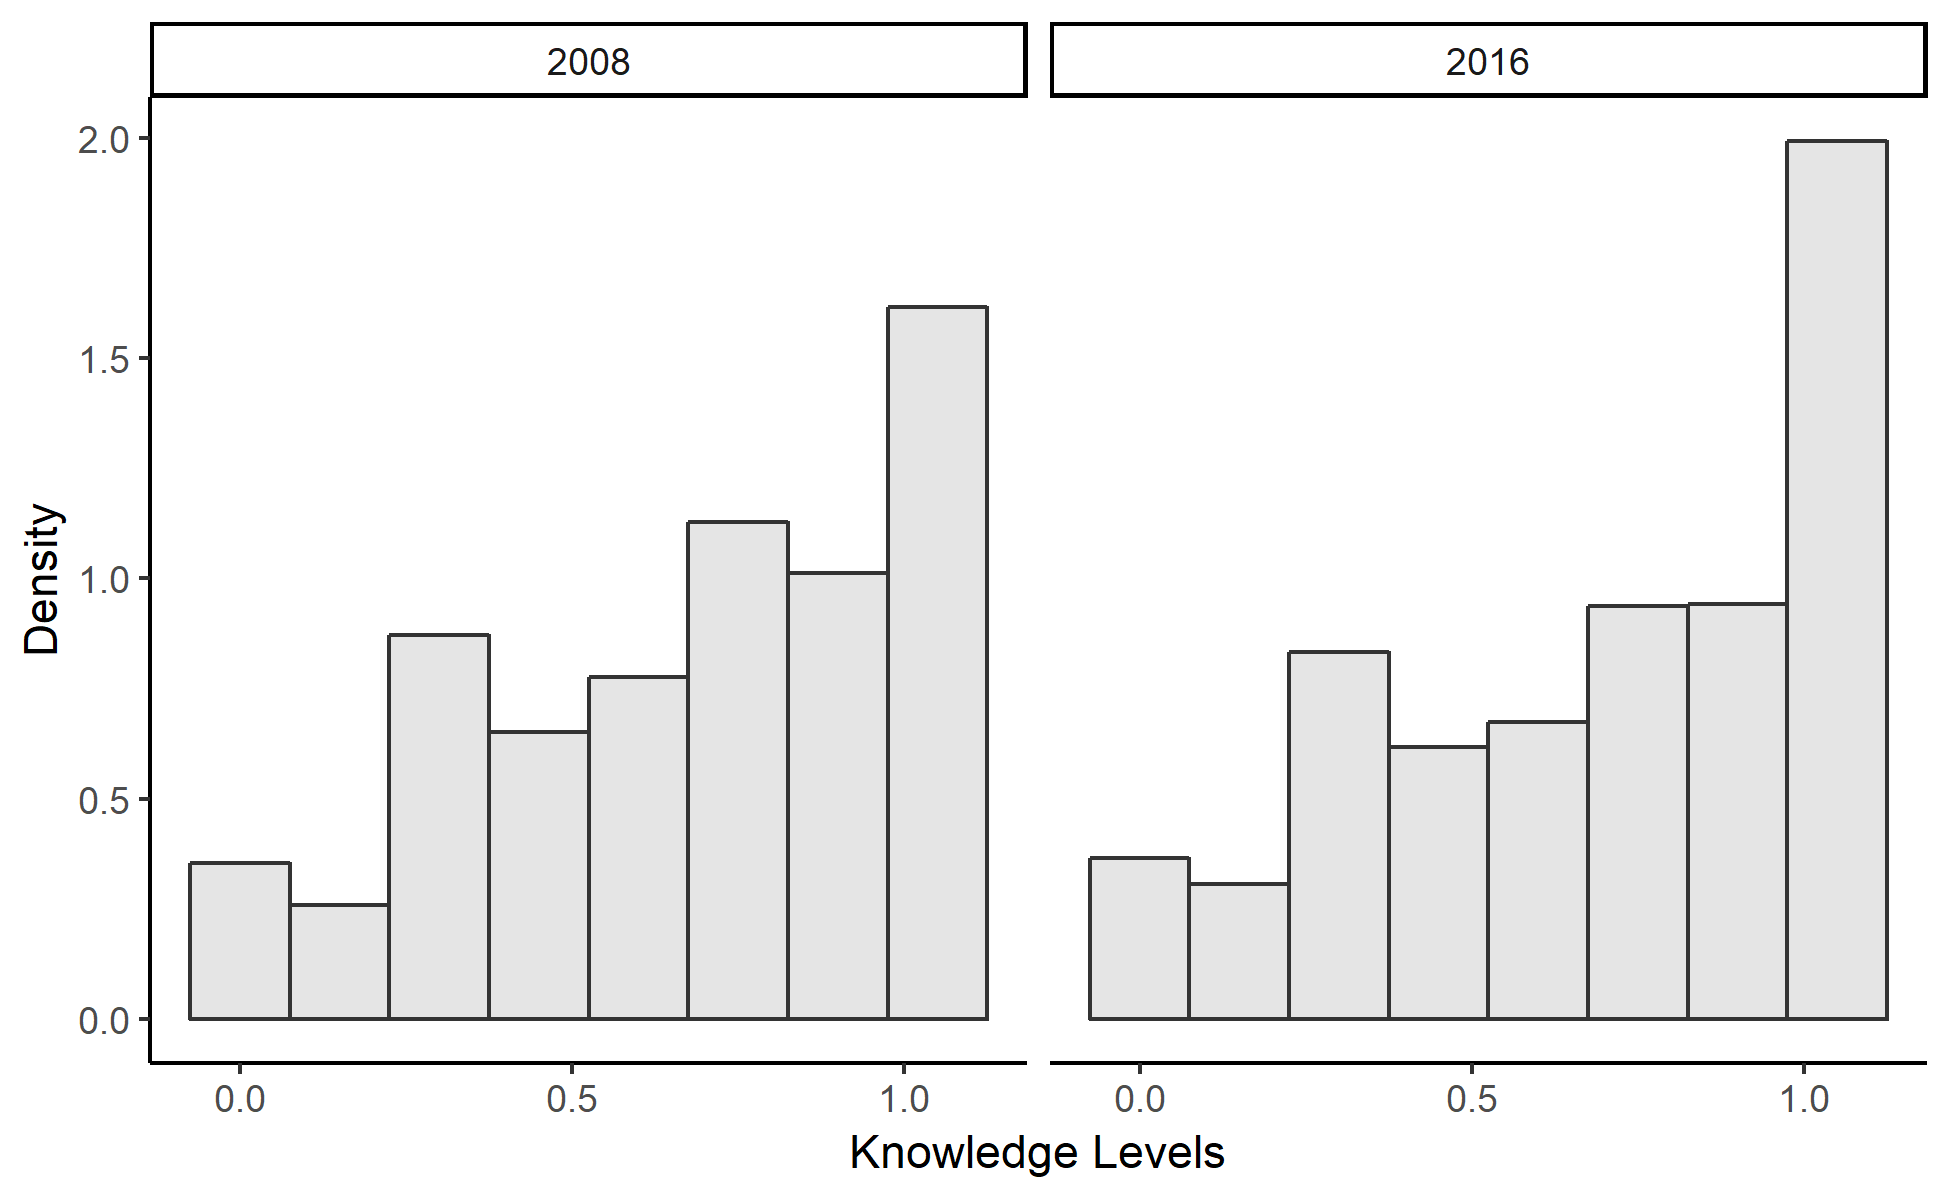
\includegraphics[width=\linewidth]{../outputs/cces_knowdist.png}
\end{figure}

\par \autoref{fig:knidxgraph2} shows the distribution of political knowledge in CCES datasets. It shows that the large portion of respondents are fully informed of the factual questions offered in the survey (political knowledge $= 1$), while there are significant numbers of respondents who are uninformed or only partially informed. The distribution of knowledge is similar across 2008 and 2016 elections, while the 2016 election involves slightly more informed respondents. Given the nature of CCES as the online survey, it should be cautioned that the absolute distribution of knowledge may not be representative of the voters in the actual election. For this study, it needed to be confirmed that there is a sufficient number of informed and uninformed voters to make a comparison of their behavioral patterns.

\begin{figure}[ht!!!]
    \caption{The distribution of local partisan environment (CCES)}
    \label{fig:pvigraph2}
    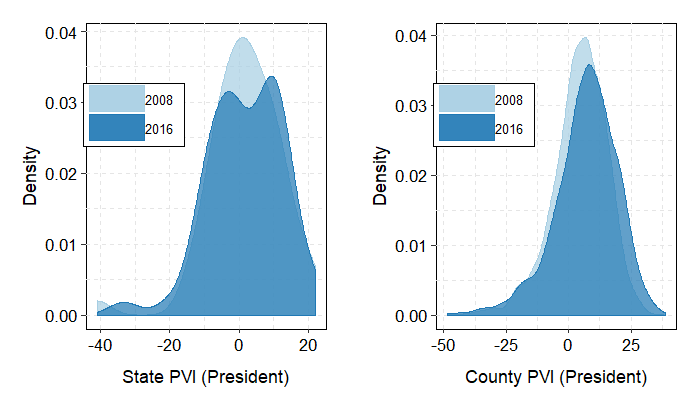
\includegraphics[width=\linewidth]{../outputs/cces_pvidist.png}
\end{figure}

\par Next, \autoref{fig:pvigraph2} shows the density distributions of local partisan environment variables. State level PVI is presented in the left-hand panel, and county level PVI is presented in right-hand panels. Those graphs show that the distributions of PVI are mostly single-peaked (with the slight exception in state PVI in 2016) and skewed to the left (there is a small number of units that are highly Democratic). It is also confirmed that significant variations exist in both state level and county level PVI. Even after adjusting for the state partisan environment, county level PVI still have a sufficient variance to explain vote choice. In fact, looking at the range of values in PVI, county PVI has a wider spread than state PVI.

\par Other variables are constructed from the following questions in CCES dataset:

\begin{itemize}
    \item Presidential vote choice (2008: \texttt{CC403} and \texttt{CC410}; 2016: \texttt{votereg\_post}, \texttt{CC16\_401} and \texttt{CC16\_410a}). 1 is voting for Republican, 0 is voting for Democrat. All other responses are dropped from the analysis.
    \item Republican advantage in squared ideological distance. Constructed from respondent's self ideology location (2008: \texttt{CC317a}; 2016: \texttt{CC16\_340a}), Republican candidate's perceived ideological location (2008: \texttt{CC317g}; 2016: \texttt{CC16\_340e}), and Democratic candidate's perceived ideological location (2008: \texttt{CC317h}; 2016: \texttt{CC16\_340d}). Each ideological position variable is rescaled in -3 to 3 range (higher score indicates more Conservative). The final variable is scaled from -36 to 36 (higher score indicates that perceived ideological position of Republican candidate is closer than the perceived ideological position of Democratic candidate to self ideology position).
    \item The retrospective evaluation of national economy (2008: \texttt{CC302}; 2016: \texttt{CC16\_302}). In 2008, the variable is scaled from gotten much worse (-2) to gotten much better (2). ``Not sure'' is recoded to 0. The scale in 2016 is reverse scaled so higher score advantages Republican candidate.   
    \item Party identity (2008: \texttt{CC307a}; 2016: \texttt{pid7}). Scaled from strong Democrat (-3) to strong Republican (3). ``Not sure'' is recoded to 0.
    \item Gender (2008: \texttt{V208}; 2016: \texttt{gender}). 1 is female and 0 is male.
    \item Age (2008: \texttt{V207}; 2016: \texttt{birthyr}).
    \item Race (2008: \texttt{V211}; 2016: \texttt{race}). Dummy variables are created for White, Black, Latino, Asian, and other races.
    \item Family income (2008: \texttt{V246}; 2016: \texttt{faminc}).
    \item Education (2008: \texttt{V213}; 2016: \texttt{educ}).
    \item Born-again Christian (2008: \texttt{V215}; 2016: \texttt{pew\_bornagain}).
\end{itemize}

\clearpage
\subsection{Detailed Logistic Regression Tables} 

\par Following tables show the full set of models estimated in CCES dataset. For both 2008 and 2016, Model 3 is used as the final model presented in the main text.

\begin{table}[ht!!!]
    \footnotesize
    \centering
    \caption{2008 Presidential Vote Choice (CCES: Republican=1, Democrat=0)}
    
\begin{tabular}{l D{)}{)}{13)3} D{)}{)}{13)3} D{)}{)}{13)3} }
\toprule
 & \multicolumn{1}{c}{Model 1} & \multicolumn{1}{c}{Model 2} & \multicolumn{1}{c}{Model 3} \\
\midrule
(Intercept)                        & -0.913 \; (0.088)^{***} & -0.423 \; (0.188)^{*}   & -0.169 \; (0.707)       \\
Knowledge                          & 1.040 \; (0.103)^{***}  & 1.054 \; (0.296)^{***}  & -0.030 \; (0.949)       \\
State PVI (By 10\%)                & 0.730 \; (0.100)^{***}  & 0.720 \; (0.121)^{***}  & 0.655 \; (0.148)^{***}  \\
County PVI (By 10\%)               & 0.435 \; (0.059)^{***}  & 0.346 \; (0.088)^{***}  & 0.149 \; (0.076)^{*}    \\
Knowledge*State PVI                & -0.481 \; (0.117)^{***} & -0.746 \; (0.160)^{***} & -0.735 \; (0.186)^{***} \\
Knowledge*County PVI               & -0.020 \; (0.065)       & -0.224 \; (0.136)       & -0.114 \; (0.115)       \\
Ideological Advantage              &                         & 0.107 \; (0.014)^{***}  & 0.108 \; (0.014)^{***}  \\
Retrospective Economic Evaluation  &                         & -0.117 \; (0.116)       & -0.021 \; (0.110)       \\
Partisanship                       &                         & 0.721 \; (0.046)^{***}  & 0.654 \; (0.042)^{***}  \\
Knowledge*Ideological Advantage    &                         & 0.233 \; (0.020)^{***}  & 0.239 \; (0.021)^{***}  \\
Knowledge*Retrospective Evaluation &                         & 1.090 \; (0.186)^{***}  & 1.100 \; (0.183)^{***}  \\
Knowledge*Partisanship             &                         & -0.189 \; (0.063)^{**}  & -0.111 \; (0.064)       \\
Female                             &                         &                         & 0.005 \; (0.150)        \\
Age                                &                         &                         & -0.958 \; (2.959)       \\
Age Squared                        &                         &                         & 2.876 \; (3.349)        \\
Black                              &                         &                         & -5.093 \; (0.915)^{***} \\
Latino                             &                         &                         & -1.190 \; (0.298)^{***} \\
Asian                              &                         &                         & -0.254 \; (0.620)       \\
Other Race                         &                         &                         & -1.256 \; (0.423)^{**}  \\
Income                             &                         &                         & 0.305 \; (0.370)        \\
Education                          &                         &                         & -0.635 \; (0.351)       \\
Born-Again Christian               &                         &                         & 0.473 \; (0.177)^{**}   \\
Knowledge*Female                   &                         &                         & 0.621 \; (0.229)^{**}   \\
Knowledge*Age                      &                         &                         & 4.859 \; (4.131)        \\
Knowledge*Age Squared              &                         &                         & -5.714 \; (4.670)       \\
Knowledge*Black                    &                         &                         & 2.708 \; (1.191)^{*}    \\
Knowledge*Latino                   &                         &                         & 1.263 \; (0.494)^{*}    \\
Knowledge*Asian                    &                         &                         & -0.626 \; (1.015)       \\
Knowledge*Other Race               &                         &                         & 1.833 \; (0.524)^{***}  \\
Knowledge*Income                   &                         &                         & -0.335 \; (0.569)       \\
Knowledge*Education                &                         &                         & -0.032 \; (0.481)       \\
Knowledge*Born-Again Christian     &                         &                         & -0.185 \; (0.217)       \\
\midrule
AIC                                & 35422.565               & 9284.096                & 8509.631                \\
BIC                                & 35470.975               & 9380.916                & 8767.819                \\
Log Likelihood                     & -17705.283              & -4630.048               & -4222.816               \\
Deviance                           & 28030.919               & 7734.934                & 6961.932                \\
Num. obs.                          & 23585                   & 23585                   & 23585                   \\
\bottomrule
\multicolumn{4}{l}{\scriptsize{$^{***}p<0.001$, $^{**}p<0.01$, $^*p<0.05$}}
\end{tabular}

\end{table}

\begin{table}[ht!!!]
    \footnotesize
    \centering
    \caption{2016 Presidential Vote Choice (CCES: Republican=1, Democrat=0)}
    
\begin{tabular}{l D{)}{)}{13)3} D{)}{)}{13)3} D{)}{)}{13)3} }
\toprule
 & \multicolumn{1}{c}{Model 1} & \multicolumn{1}{c}{Model 2} & \multicolumn{1}{c}{Model 3} \\
\midrule
(Intercept)                        & -0.117 \; (0.099)      & 0.237 \; (0.104)^{*}    & -0.180 \; (0.588)       \\
Knowledge                          & 0.093 \; (0.102)       & -1.098 \; (0.139)^{***} & -0.512 \; (0.931)       \\
State PVI (By 10\%)                & 0.537 \; (0.117)^{***} & 0.425 \; (0.133)^{**}   & 0.374 \; (0.123)^{**}   \\
County PVI (By 10\%)               & 0.461 \; (0.041)^{***} & 0.331 \; (0.045)^{***}  & 0.183 \; (0.050)^{***}  \\
Knowledge*State PVI                & -0.146 \; (0.118)      & -0.479 \; (0.163)^{**}  & -0.458 \; (0.159)^{**}  \\
Knowledge*County PVI               & -0.089 \; (0.046)      & -0.185 \; (0.059)^{**}  & -0.105 \; (0.064)       \\
Ideological Alignment              &                        & 0.067 \; (0.006)^{***}  & 0.069 \; (0.006)^{***}  \\
Partisanship                       &                        & 0.662 \; (0.041)^{***}  & 0.601 \; (0.039)^{***}  \\
Retrospective Economic Evaluation  &                        & 0.246 \; (0.081)^{**}   & 0.286 \; (0.076)^{***}  \\
Knowledge*Ideological Alignment    &                        & 0.133 \; (0.010)^{***}  & 0.128 \; (0.009)^{***}  \\
Knowledge*Partisanship             &                        & 0.017 \; (0.054)        & 0.058 \; (0.052)        \\
Knowledge*Retrospective Evaluation &                        & 1.052 \; (0.112)^{***}  & 1.030 \; (0.121)^{***}  \\
Female                             &                        &                         & -0.849 \; (0.126)^{***} \\
Age                                &                        &                         & 5.086 \; (2.667)        \\
Age Squared                        &                        &                         & -4.982 \; (2.736)       \\
Black                              &                        &                         & -2.081 \; (0.350)^{***} \\
Latino                             &                        &                         & -1.388 \; (0.316)^{***} \\
Asian                              &                        &                         & -1.092 \; (0.316)^{***} \\
Other Race                         &                        &                         & -0.948 \; (0.243)^{***} \\
Income                             &                        &                         & 1.252 \; (0.352)^{***}  \\
Education                          &                        &                         & -0.832 \; (0.247)^{***} \\
Born-Again Christian               &                        &                         & 0.723 \; (0.141)^{***}  \\
Knowledge*Female                   &                        &                         & 0.385 \; (0.189)^{*}    \\
Knowledge*Age                      &                        &                         & -2.394 \; (3.715)       \\
Knowledge*Age Squared              &                        &                         & 2.170 \; (3.615)        \\
Knowledge*Black                    &                        &                         & 0.579 \; (0.655)        \\
Knowledge*Latino                   &                        &                         & 0.894 \; (0.758)        \\
Knowledge*Asian                    &                        &                         & 0.805 \; (0.413)        \\
Knowledge*Other Race               &                        &                         & 0.948 \; (0.399)^{*}    \\
Knowledge*Income                   &                        &                         & -1.399 \; (0.470)^{**}  \\
Knowledge*Education                &                        &                         & 0.008 \; (0.333)        \\
Knowledge*Born-Again Christian     &                        &                         & -0.379 \; (0.167)^{*}   \\
\midrule
AIC                                & 54029.263              & 15960.343               & 15024.881               \\
BIC                                & 54080.967              & 16063.750               & 15300.633               \\
Log Likelihood                     & -27008.632             & -7968.171               & -7480.440               \\
Deviance                           & 53681.964              & 16082.617               & 15075.333               \\
Num. obs.                          & 40834                  & 40834                   & 40834                   \\
\bottomrule
\multicolumn{4}{l}{\scriptsize{$^{***}p<0.001$, $^{**}p<0.01$, $^*p<0.05$}}
\end{tabular}

\end{table}

\clearpage

\section{Study 2 Appendix} \label{appB}
\setcounter{table}{0}
\renewcommand{\thetable}{B\arabic{table}}
\setcounter{figure}{0}
\renewcommand{\thefigure}{B\arabic{figure}}

\subsection{Variable Constructs}

\par Most of the variables for analysis are extracted from ANES 1948-2016 cumulative data file (downloaded on April 22, 2019). The original code name of the variable refers to the cumulative file unless specified otherwise. 

\par To start with, interviewer's rating of knowledge is constructed using \texttt{vcf0050a}. The original question asks interviewers to assess ``respondent's general level of information about politics and public affairs.'' Answers are converted to the number by following the scheme used in \cite{Bartels1996unvo}, as follows:
\begin{itemize}
    \item Very High = 0.95
    \item Fairly High = 0.80
    \item Average = 0.50
    \item Fairly Low = 0.20
    \item Very Low = 0.05
\end{itemize}    
\noindent In \cite{Bartels1996unvo}, then, the hypothetical individual with the value 1 is defined as informed, and the hypothetical individual with value 0 is defined as uninformed.

\begin{figure}[ht!!!]
    \caption{The distribution of interviewer's rating of knowledge (1972-2016)}
    \label{fig:anes_sbjkndist}
    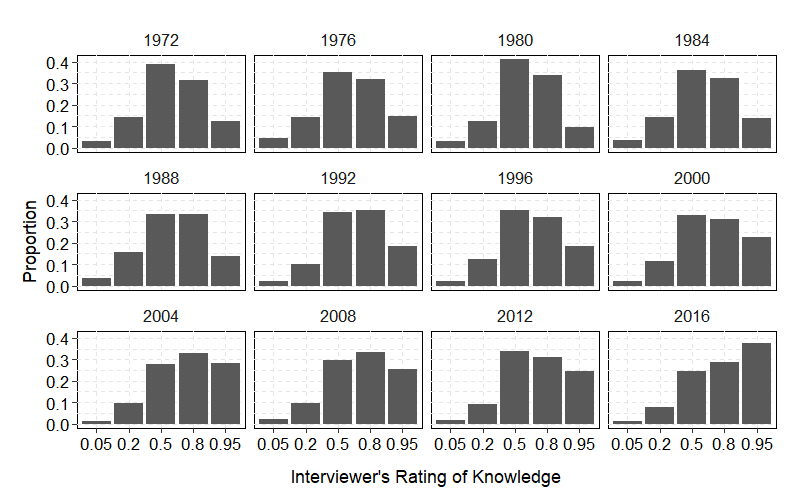
\includegraphics[width=\linewidth]{../outputs/anes_sbjkndist.png}
\end{figure}

\par \autoref{fig:anes_sbjkndist} shows the distribution of interviewer's rating of knowledge at each presidential election year of ANES time-series studies. The distribution is approximately normal for most of the early years, but the average level of knowledge is gradually over the years. In 2016, the distribution had the mode at 0.95. As a result, the knowledge distribution in 2008 and 2016 are similar to that of CCES knowledge score.    

\par Other variables are constructed from the following questions in ANES dataset:

\begin{itemize}
    \item Presidential vote choice (\texttt{vcf0704}). 1 is voting for Republican, 0 is voting for Democrat. All other responses are dropped from the analysis.
    \item Republican advantage in squared ideological distance. Constructed from respondent's self ideology location (\texttt{vcf0803}, \texttt{V720652} from 1972 data, \texttt{V763286} from 1976 data, \texttt{V800267} from 1980 data, \texttt{V840370} from 1984 data, \texttt{v000440} from 2000 data, and \texttt{v162171} and \texttt{v162171a} from 2016 data), Republican candidate's perceived ideological location (\texttt{vcf9096}), and Democratic candidate's perceived ideological location (\texttt{vcf9088}). Each ideological position variable is rescaled in -3 to 3 range (higher score indicates more Conservative). The final variable is scaled from -36 to 36 (higher score indicates that perceived ideological position of Republican candidate is closer than the perceived ideological position of Democratic candidate to self ideology position).
    \item The retrospective evaluation of national economy (\texttt{vcf0870}, \texttt{vcf0871}, \texttt{v720780} from 1972 data, and \texttt{v763139} from 1976 data). The variable is scaled from gotten much worse (-2) to gotten much better (2). The scale in election years with Democratic party as incumbent is reverse scaled so higher score advantages Republican candidate. 
    \item Party identity (\texttt{vcf0301}). Scaled from strong Democrat (-2) to strong Republican (2).
    \item Gender (\texttt{vcf0104}). 1 is female and 0 is male.
    \item Age (\texttt{vcf0101}).
    \item Race (\texttt{vcf0106}). Dummy variable is created for ethnic minority (i.e., non-White) respondents.
    \item Family income (\texttt{v720420} from 1972 data, \texttt{v763507} from 1976 data, \texttt{v800686} from 1980 data, \texttt{v840680} from 1984 data, \texttt{v880520} from 1988 data, \texttt{v924104} from 1992 data, \texttt{v960701} from 1996 data, \texttt{v000994} from 2000 data, \texttt{v04329x} from 2004 data, \texttt{v083248x} from 2008 data, \texttt{incgroup\_prepost\_x} from 2012 data, and \texttt{v161361x} and \texttt{v162309x} from 2016 data). Rescaled as a percentile.
    \item Education (\texttt{v720300} from 1972 data, \texttt{v763389} from 1976 data, \texttt{v800436} from 1980 data, \texttt{v840438} from 1984 data, \texttt{v880422} from 1988 data, \texttt{v923905} and \texttt{923908} from 1992 data, \texttt{v960607} and \texttt{960610} from 1996 data, \texttt{v000913} from 2000 data, \texttt{v043254} from 2004 data, \texttt{v083218x} from 2008 data, \texttt{dem\_edu} from 2012 data, and \texttt{vV161270} from 2016 data). Converted to the scale from 0 to 17.
    \item Religion (\texttt{vcf0128}, \texttt{v161247a} and \texttt{v161247b} from 2016 data). Creating dummy variables for Protestant and Catholic.
\end{itemize}

\subsection{Results for Demographic Controls} 

\par Following figures show the conditional coefficients of demographic control variables on the presidential vote choice (i.e., 1 = vote Republican, 0 = vote Democratic) in each presidential election year. Coefficients for individual preference variables are included in the main text. 

\begin{figure}[ht!!!]
    \caption{The impact of demographic variables on presidential Vote Choice (1 = Republican, 0 = Democrat) in ANES Part I (1972-2016)}
    \label{fig:anescoefplot_dem1}
    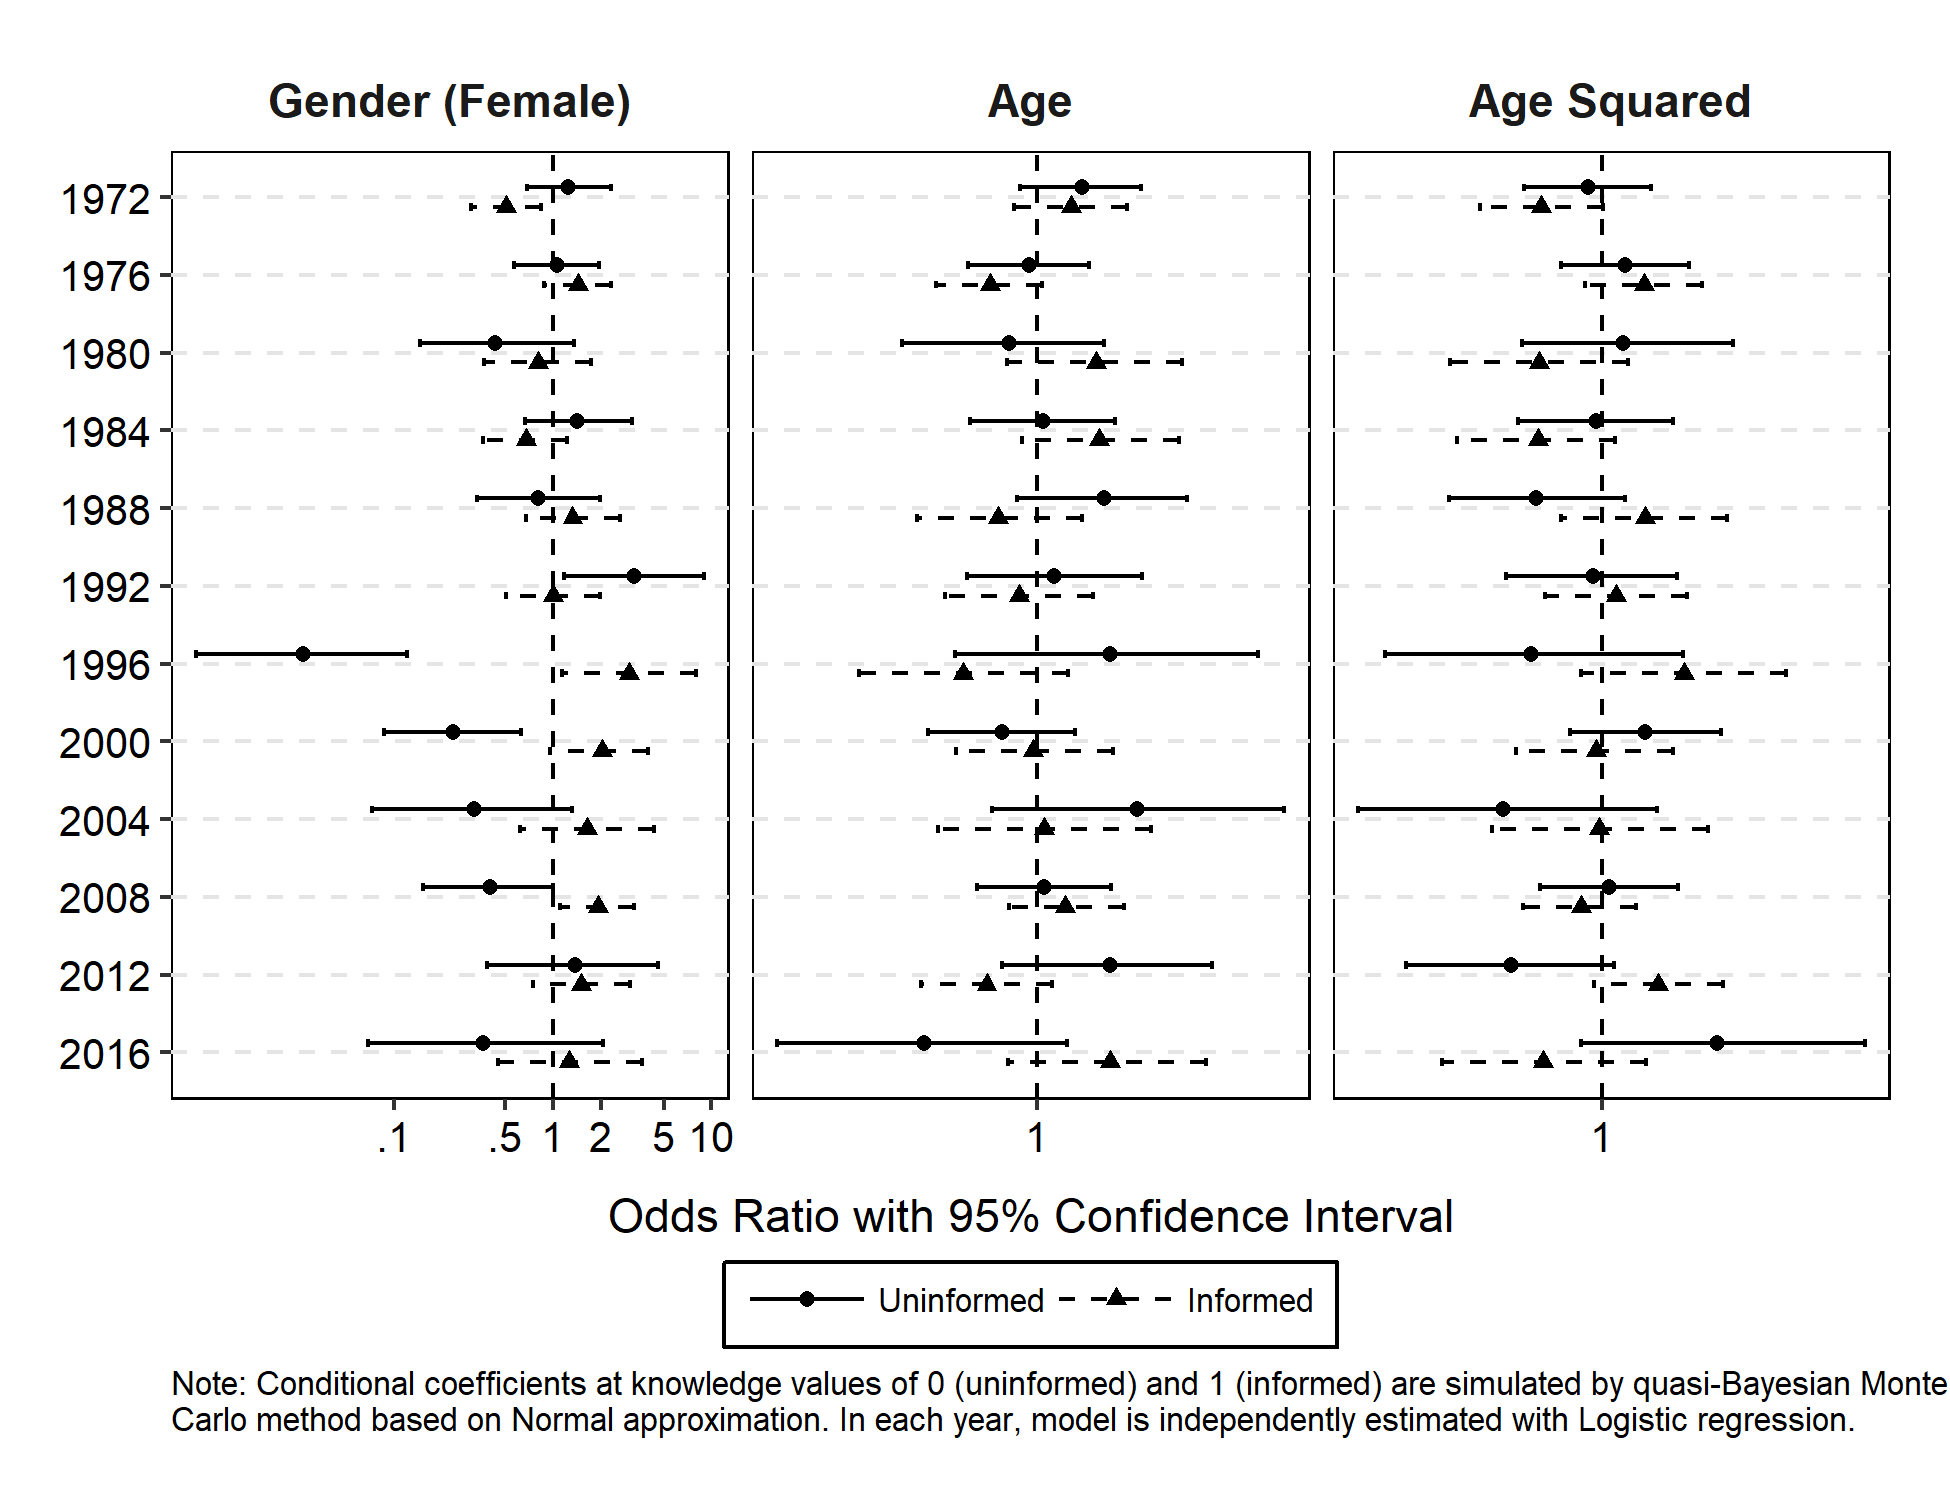
\includegraphics[width=\linewidth]{../outputs/m1sq_anescoefplot_dem1.png}
\end{figure}

\begin{figure}[ht!!!]
    \caption{The impact of demographic variables on presidential Vote Choice (1 = Republican, 0 = Democrat) in ANES Part II (1972-2016)}
    \label{fig:anescoefplot_dem2}
    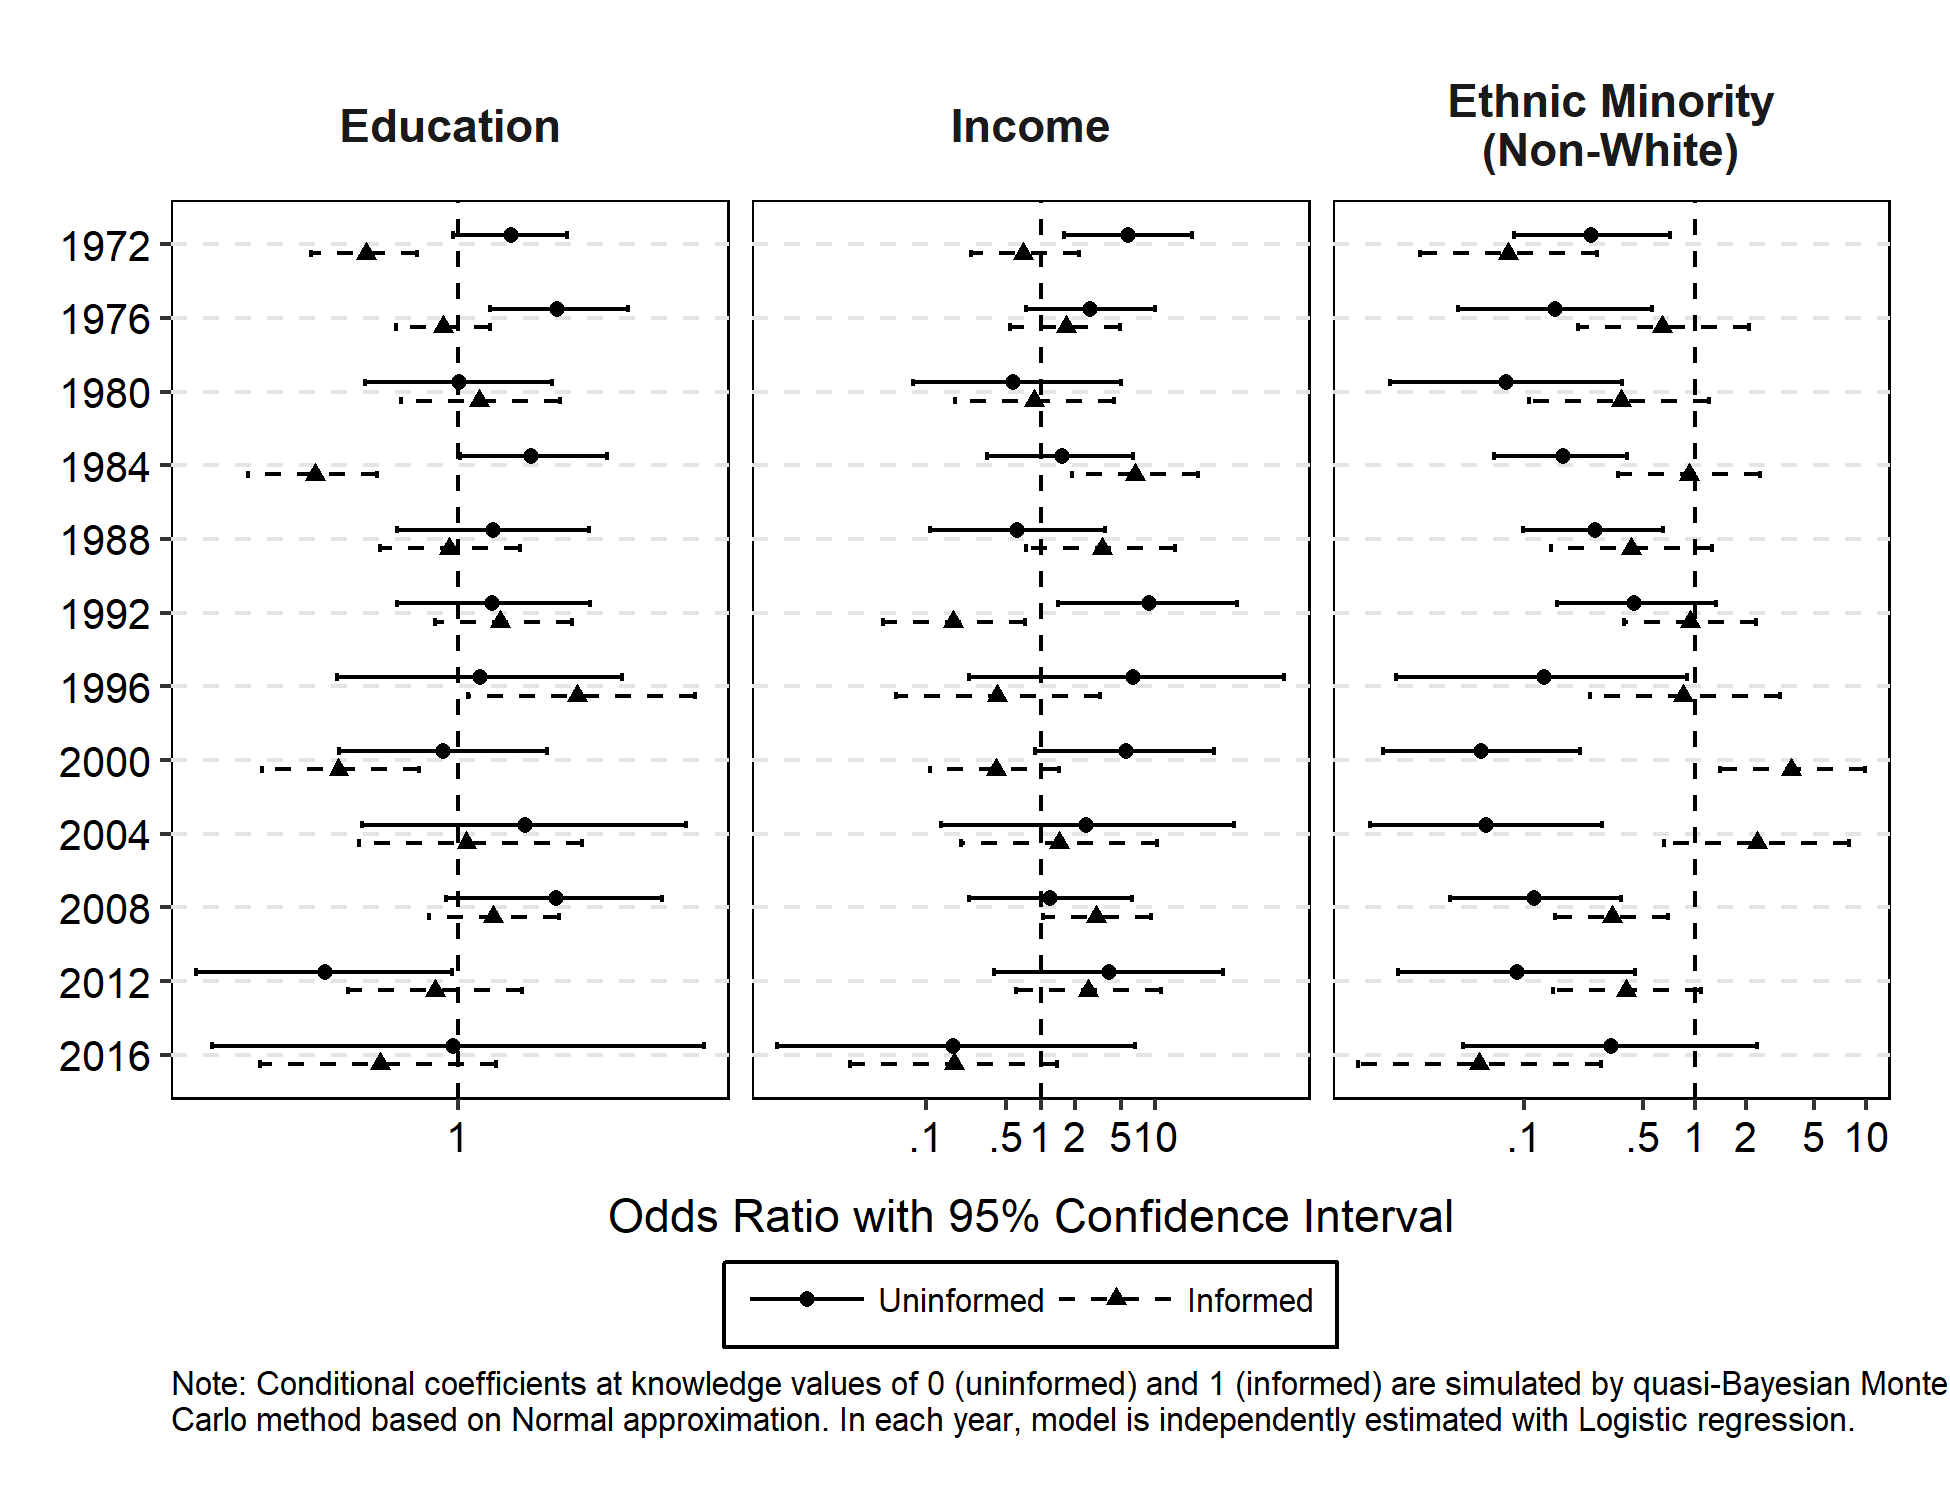
\includegraphics[width=\linewidth]{../outputs/m1sq_anescoefplot_dem2.png}
\end{figure}

\begin{figure}[ht!!!]
    \caption{The impact of demographic variables on presidential Vote Choice (1 = Republican, 0 = Democrat) in ANES Part III (1972-2016)}
    \label{fig:anescoefplot_dem3}
    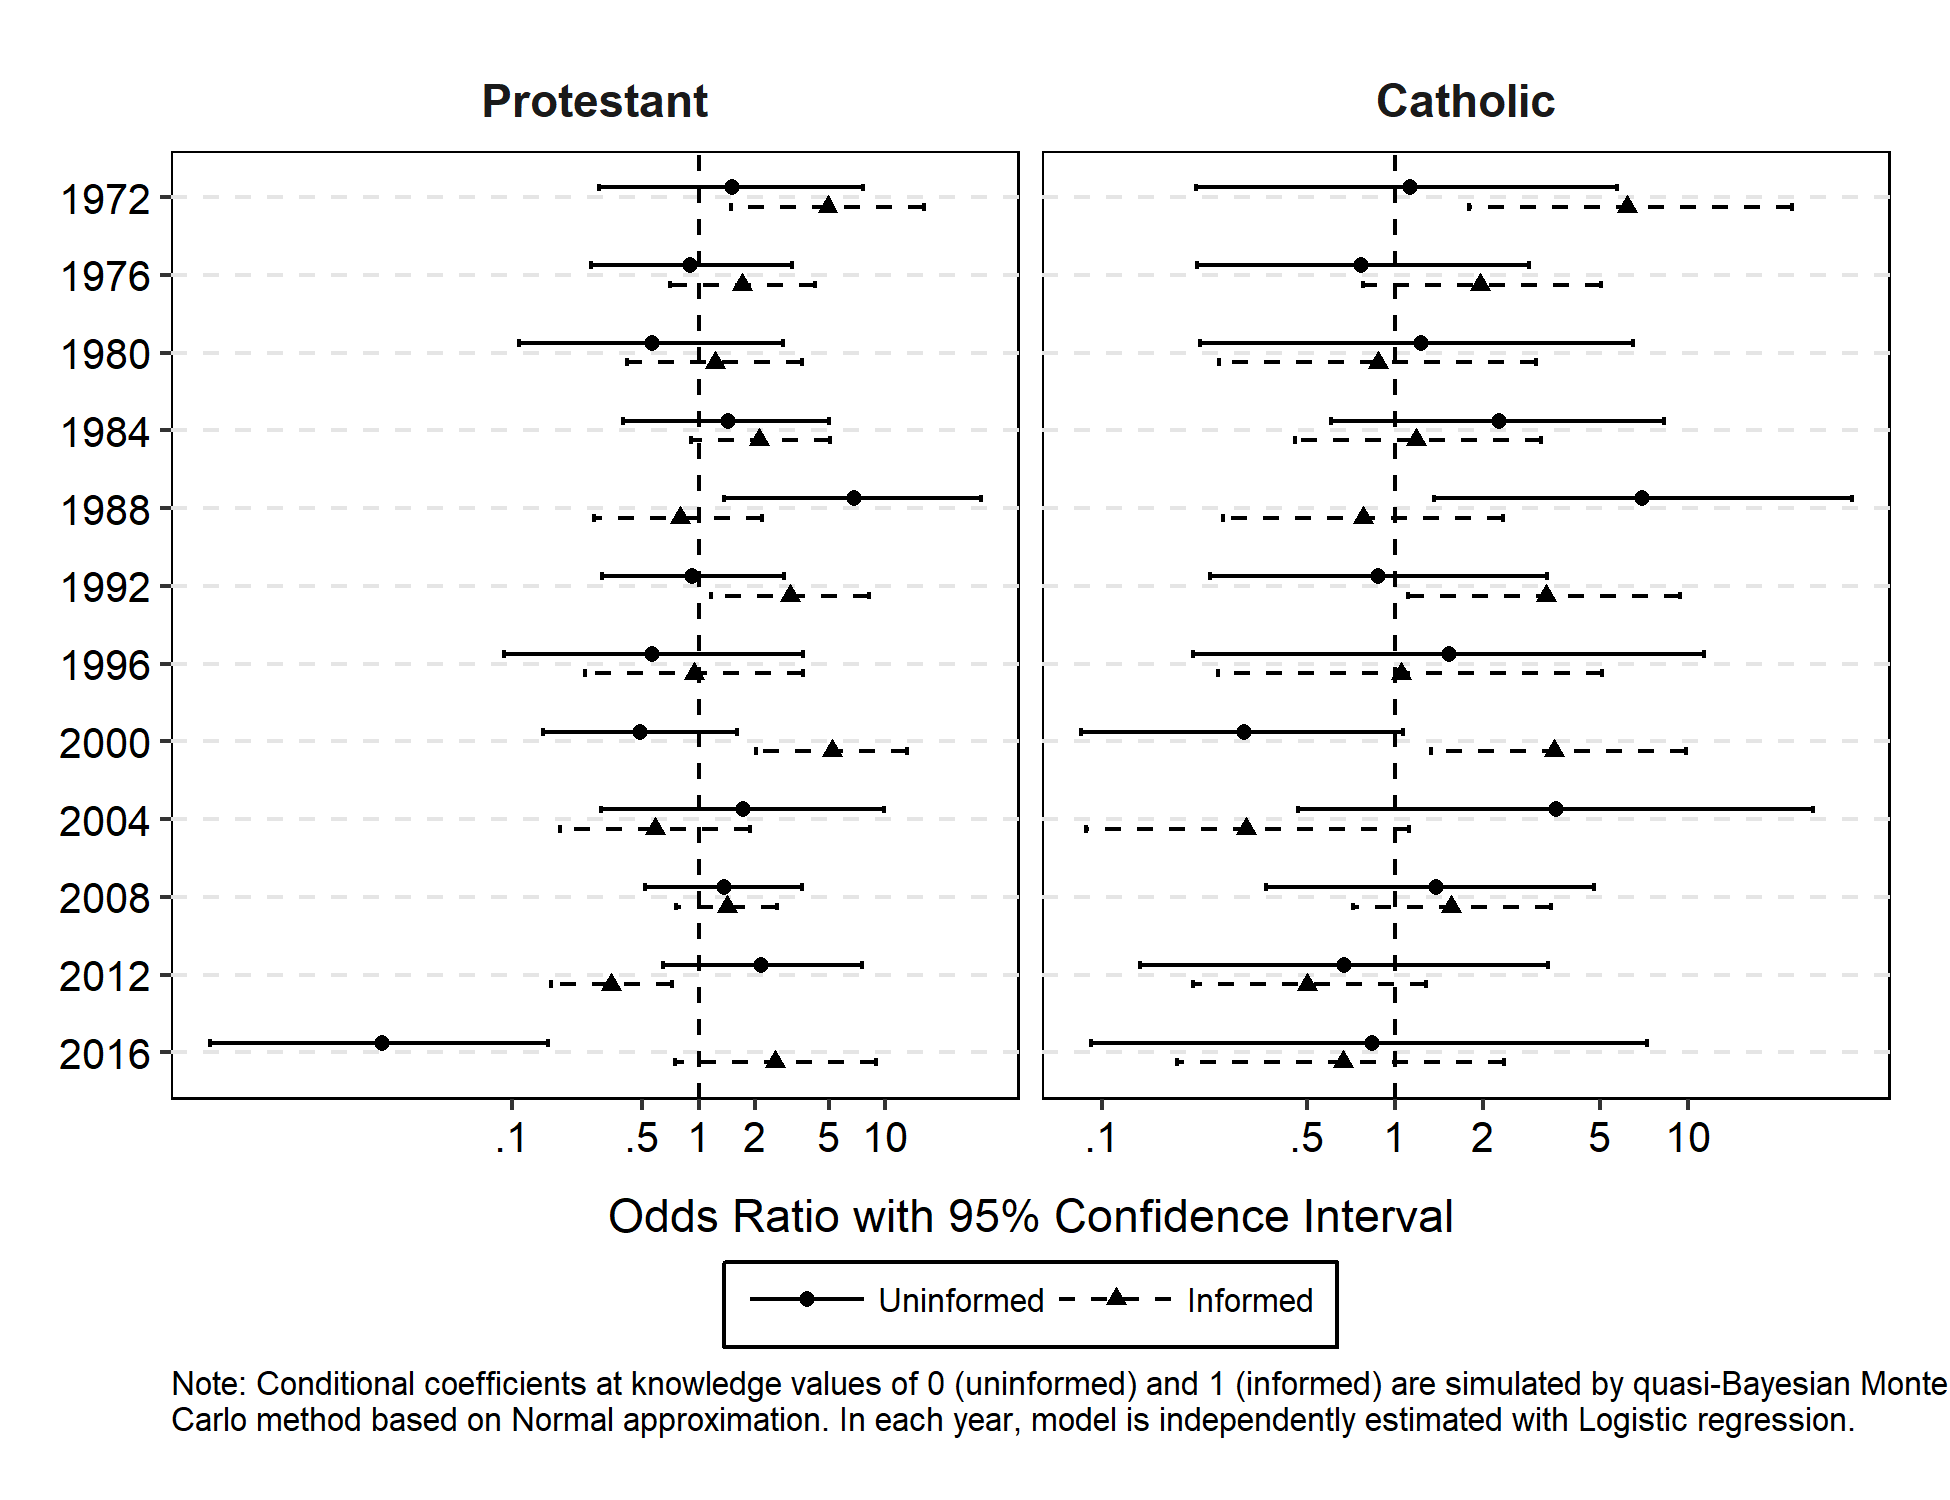
\includegraphics[width=\linewidth]{../outputs/m1sq_anescoefplot_dem3.png}
\end{figure}

\clearpage
\subsection{EDV Models Using Predictions Based on Voter Profiles from Different Years}

\begin{figure}[ht!!!]
    \caption{National partisan environment and incumbent party explain predicted probability of Republican vote in ANES (1972-2016), estimated with voter profiles from different years}
    \label{fig:anespredtable}
    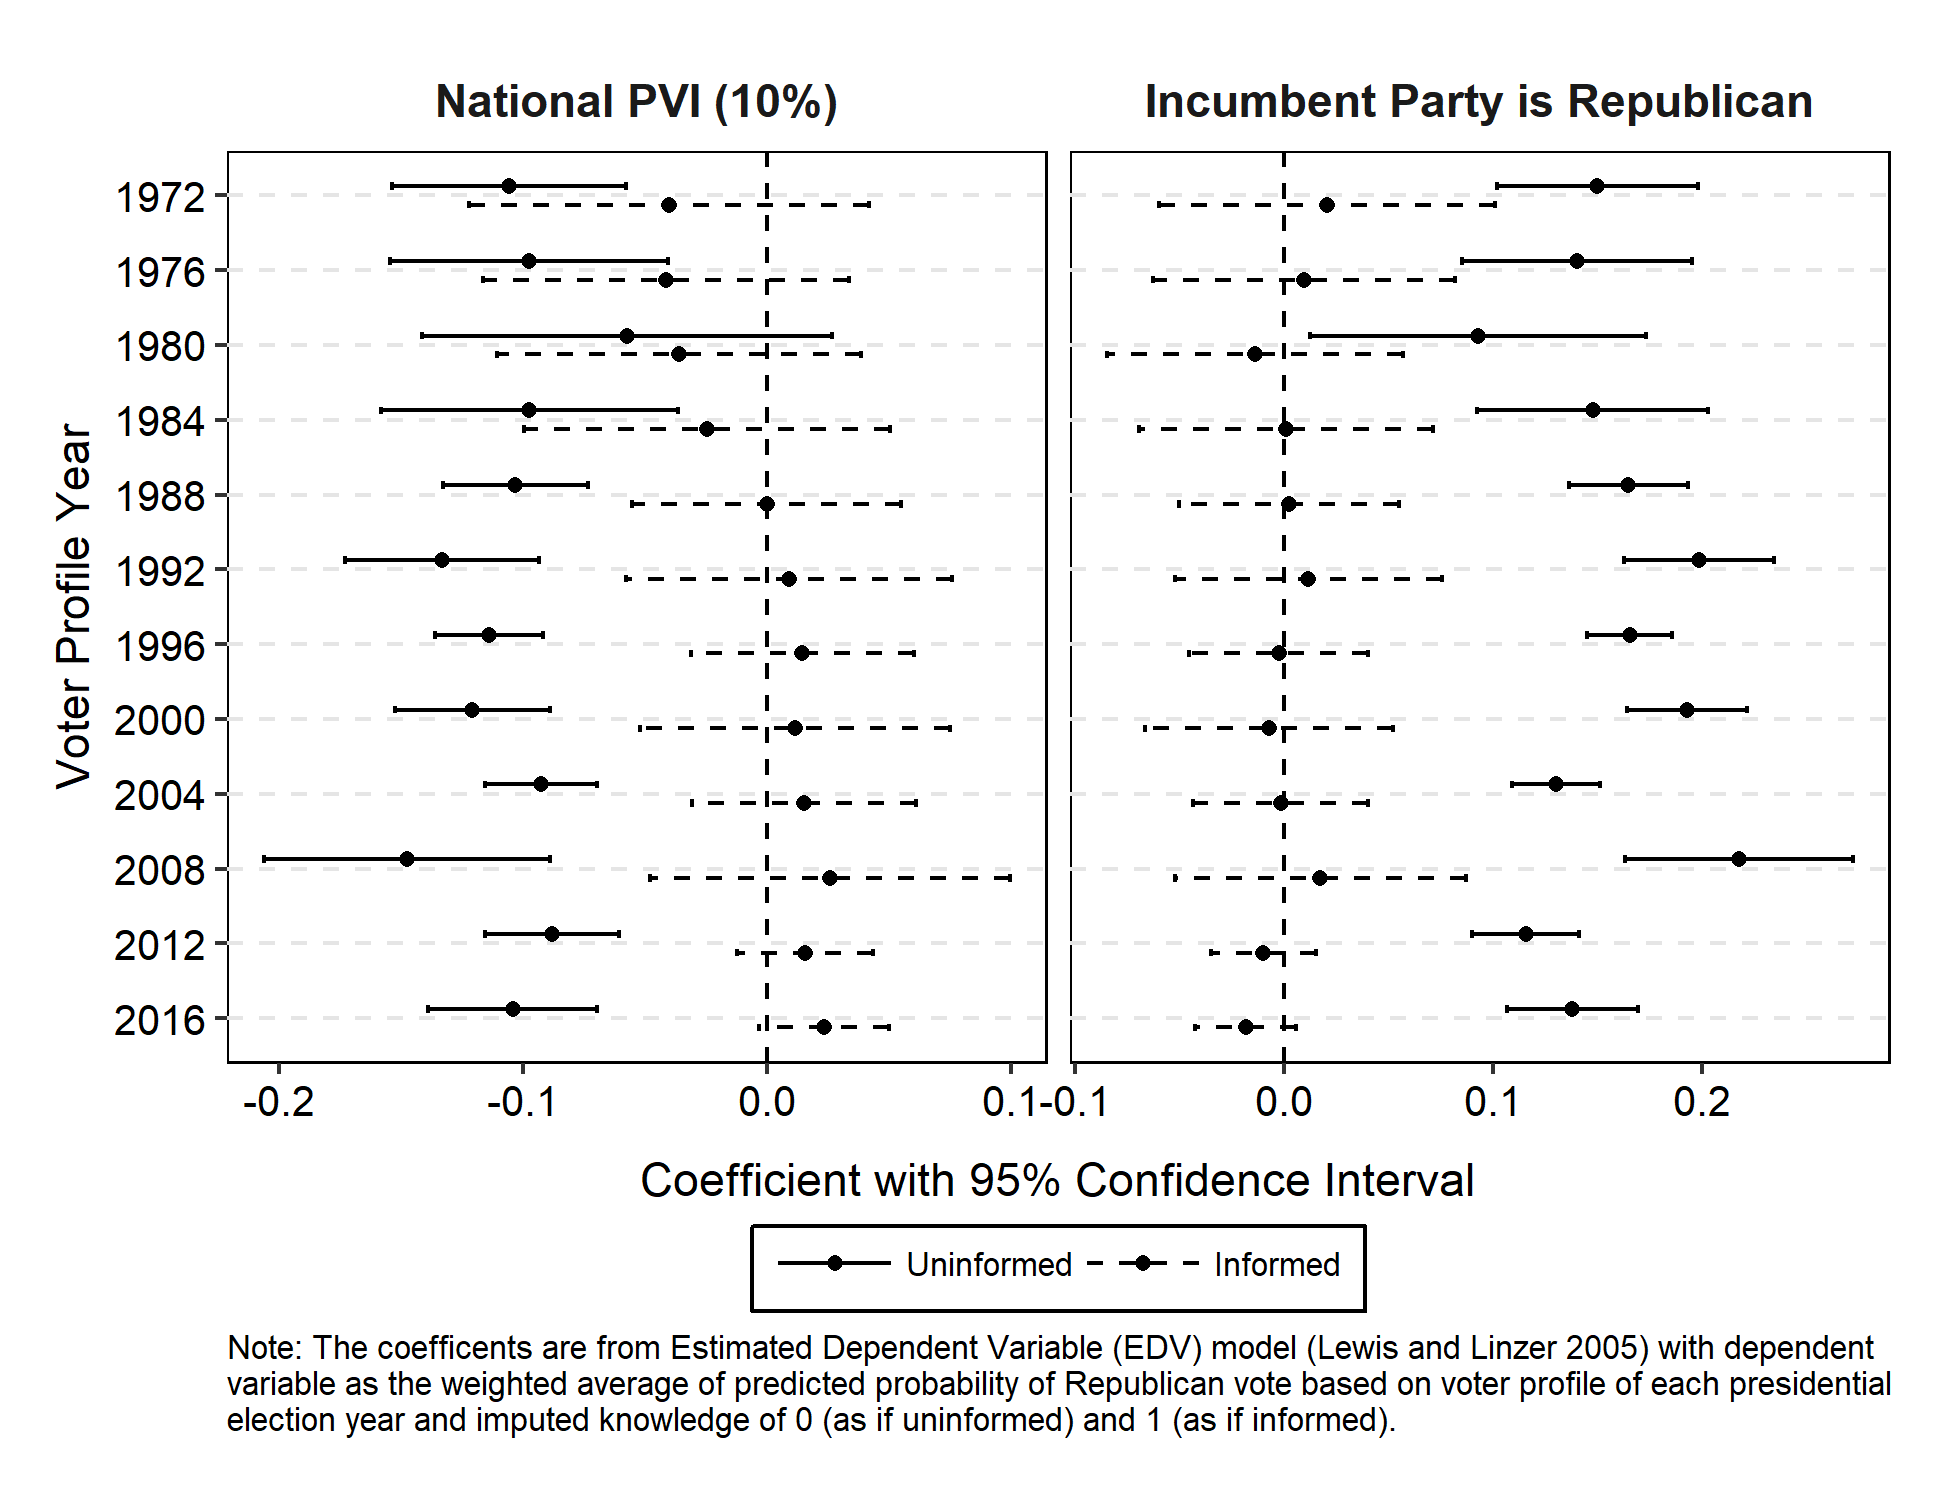
\includegraphics[width=\linewidth]{../outputs/m1sq_anespredtable.png}
\end{figure}

\par \autoref{fig:anespredtable} shows the coefficient from EDV regressions with national PVI and incumbent party (i.e., Republican = 1, Democrat = 0) as predictors. The outcome is the weighted average of the probability of Republican vote based on the voter profile from the given year and manipulated value of knowledge (i.e., either 0 = uninformed or 1 = informed). The result confirms that national PVI has a negative influence on the predicted Republican vote probability of uninformed voters with the voter profile from any given year (the coefficient is statistically significant at 5\% level for all but 1980 profile). Similarly, Republican being incumbent party has a consistently positive impact on the Republican vote probability of uninformed voters. On the other hand, two variables are never significant predictors of Republican voter probability of informed voters.        

\clearpage
\subsection{Analysis with Objective Knowledge}

\par The objective knowledge score from ANES is constructed from aggregating correct answers to following questions offered in each election year. 

\begin{itemize}
    \item 1972: \texttt{v720943}, \texttt{v720944}, \texttt{v720945}, \texttt{v720946a}, \texttt{v720947a}, \texttt{v720946b}, \texttt{v720947b}, \texttt{v720948}, \texttt{v720949}, \texttt{v720950}, and \texttt{v720951}  (\texttt{v720006} to code correct answer)
    \item 1976: \texttt{v763683} and \texttt{v763684}
    \item 1980: \texttt{v801028}, \texttt{v801029}, \texttt{v800826}, \texttt{v800829}, \texttt{v800913} (\texttt{v800823} is used to identify missing values, \texttt{vcf0977} and \texttt{vcf0978} from cumulative data are used to code correct answers)
    \item 1984: \texttt{v841006}, \texttt{v841007}, \texttt{v840741}, \texttt{v840745}, and \texttt{v840741} (\texttt{v840737} is used to identify missing values, \texttt{vcf0977} and \texttt{vcf0978} from cumulative data are used to code correct answers)
    \item 1988: \texttt{v880878}, \texttt{v880569}, \texttt{v880573}, \texttt{v880879}, \texttt{v880709}, \texttt{v880712}, \texttt{v880871}, \texttt{v880872}, \texttt{v880873}, \texttt{v880874}, \texttt{v880875}, \texttt{v880876}, and \texttt{v880877} (\texttt{v880565} is used to identify missing values, \texttt{vcf0977} and \texttt{vcf0978} from cumulative data are used to code correct answers)
    \item 1992: \texttt{v925951}, \texttt{v925113}, \texttt{v925117}, \texttt{v925952}, \texttt{v925435},\texttt{v925438}, \texttt{v925916}, \texttt{v925917}, \texttt{v925918}, \texttt{v925919}, \texttt{v925920}, and \texttt{v925921} (\texttt{v925109} is used to identify missing values, \texttt{vcf0977} and \texttt{vcf0978} from cumulative data are used to code correct answers)
    \item 1996: \texttt{v961072}, \texttt{v961010}, \texttt{v961014}, \texttt{v961073}, \texttt{v961068}, \texttt{v961070}, \texttt{v961189}, \texttt{v961190}, \texttt{v961191}, and \texttt{v961192} (\texttt{v961006} is used to identify missing values, \texttt{vcf0977} and \texttt{vcf0978} from cumulative data are used to code correct answers)
    \item 2000: \texttt{v001356}, \texttt{v001210}, \texttt{v001214}, \texttt{v001357}, \texttt{v001353a}, \texttt{v001354}, \texttt{v001447}, \texttt{v001450}, \texttt{v001453}, and \texttt{v001456} (\texttt{v001206} is used to identify missing values, \texttt{vcf0977} and \texttt{vcf0978} from cumulative data are used to code correct answers)
    \item 2004: \texttt{v045089}, \texttt{v045090}, \texttt{v045162}, \texttt{v045163}, \texttt{v045164}, and \texttt{v045165}
    \item 2008: \texttt{v085066}, \texttt{v085067}, \texttt{v085120}, \texttt{v085120}, \texttt{v085121}, \texttt{v085122}, and \texttt{v085123} (\texttt{PELOSI\_Level1}, \texttt{CHENEY\_Level1}, \texttt{BROWN\_Level1}, and \texttt{ROBERTS\_Level1} in 2008 Office Recognition Coding Data are used to code correct answers)
    \item 2012: \texttt{preknow\_prestimes}, \texttt{preknow\_sizedef}, \texttt{preknow\_senterm}, \texttt{preknow\_medicare}, \texttt{preknow\_leastsp}, \texttt{knowl\_housemaj}, \texttt{knowl\_senmaj}, \texttt{ofcrec\_speaker\_correct}, \texttt{ofcrec\_vp\_correct}, \texttt{ofcrec\_pmuk\_correct}, and \texttt{ofcrec\_cj\_correct}
    \item 2016: \texttt{v161515}, \texttt{v161516}, \texttt{v162072}, \texttt{v162073a}, \texttt{v162074a}, \texttt{162075a}, \texttt{162076a}
\end{itemize}

\noindent To generate the comparable measure of objective knowledge, I train simple one-dimensional Item Response Theory (IRT) score within each survey year. The exported score has a mean of approximately 0 and the standard deviation of 1. I rescaled the score so that it has a mean of 0.5 and a standard deviation of 0.5. The conditional coefficients are calculated by setting this variable at 0 (uninformed, 2SD below the mean) and 1 (informed, 2SD above the mean). 

\begin{figure}[ht!!!]
    \caption{The distribution of objective knowledge score (1972-2016)}
    \label{fig:anes_objkndist}
    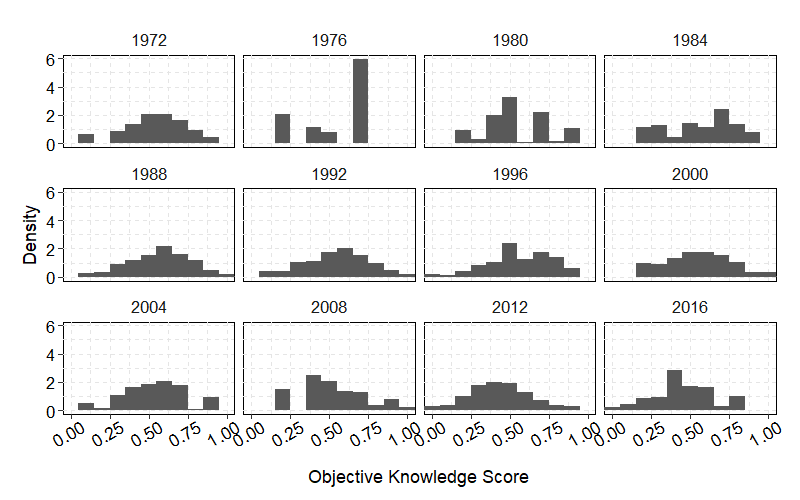
\includegraphics[width=\linewidth]{../outputs/anes_objkndist.png}
\end{figure}

\noindent \autoref{fig:anes_objkndist} shows the distribution of objective knowledge score at each given year. With the exception of 1976, the score in each year approximately looks normal. In 1976, only two factual test knowledge questions were offered, so the results should be interpreted with caution.

\par \autoref{fig:v2anescoefplot}, \autoref{fig:v2anescoefplot_dem1}, \autoref{fig:v2anescoefplot_dem2}, and \autoref{fig:v2anescoefplot_dem3} show the results of models predicting Republican vote with individual preference and demography variables. 

\begin{figure}[ht!!!]
    \caption{The impact of individual preference variables on presidential Vote Choice (1 = Republican, 0 = Democrat) in ANES (1972-2016) (objective knowledge)}
    \label{fig:v2anescoefplot}
    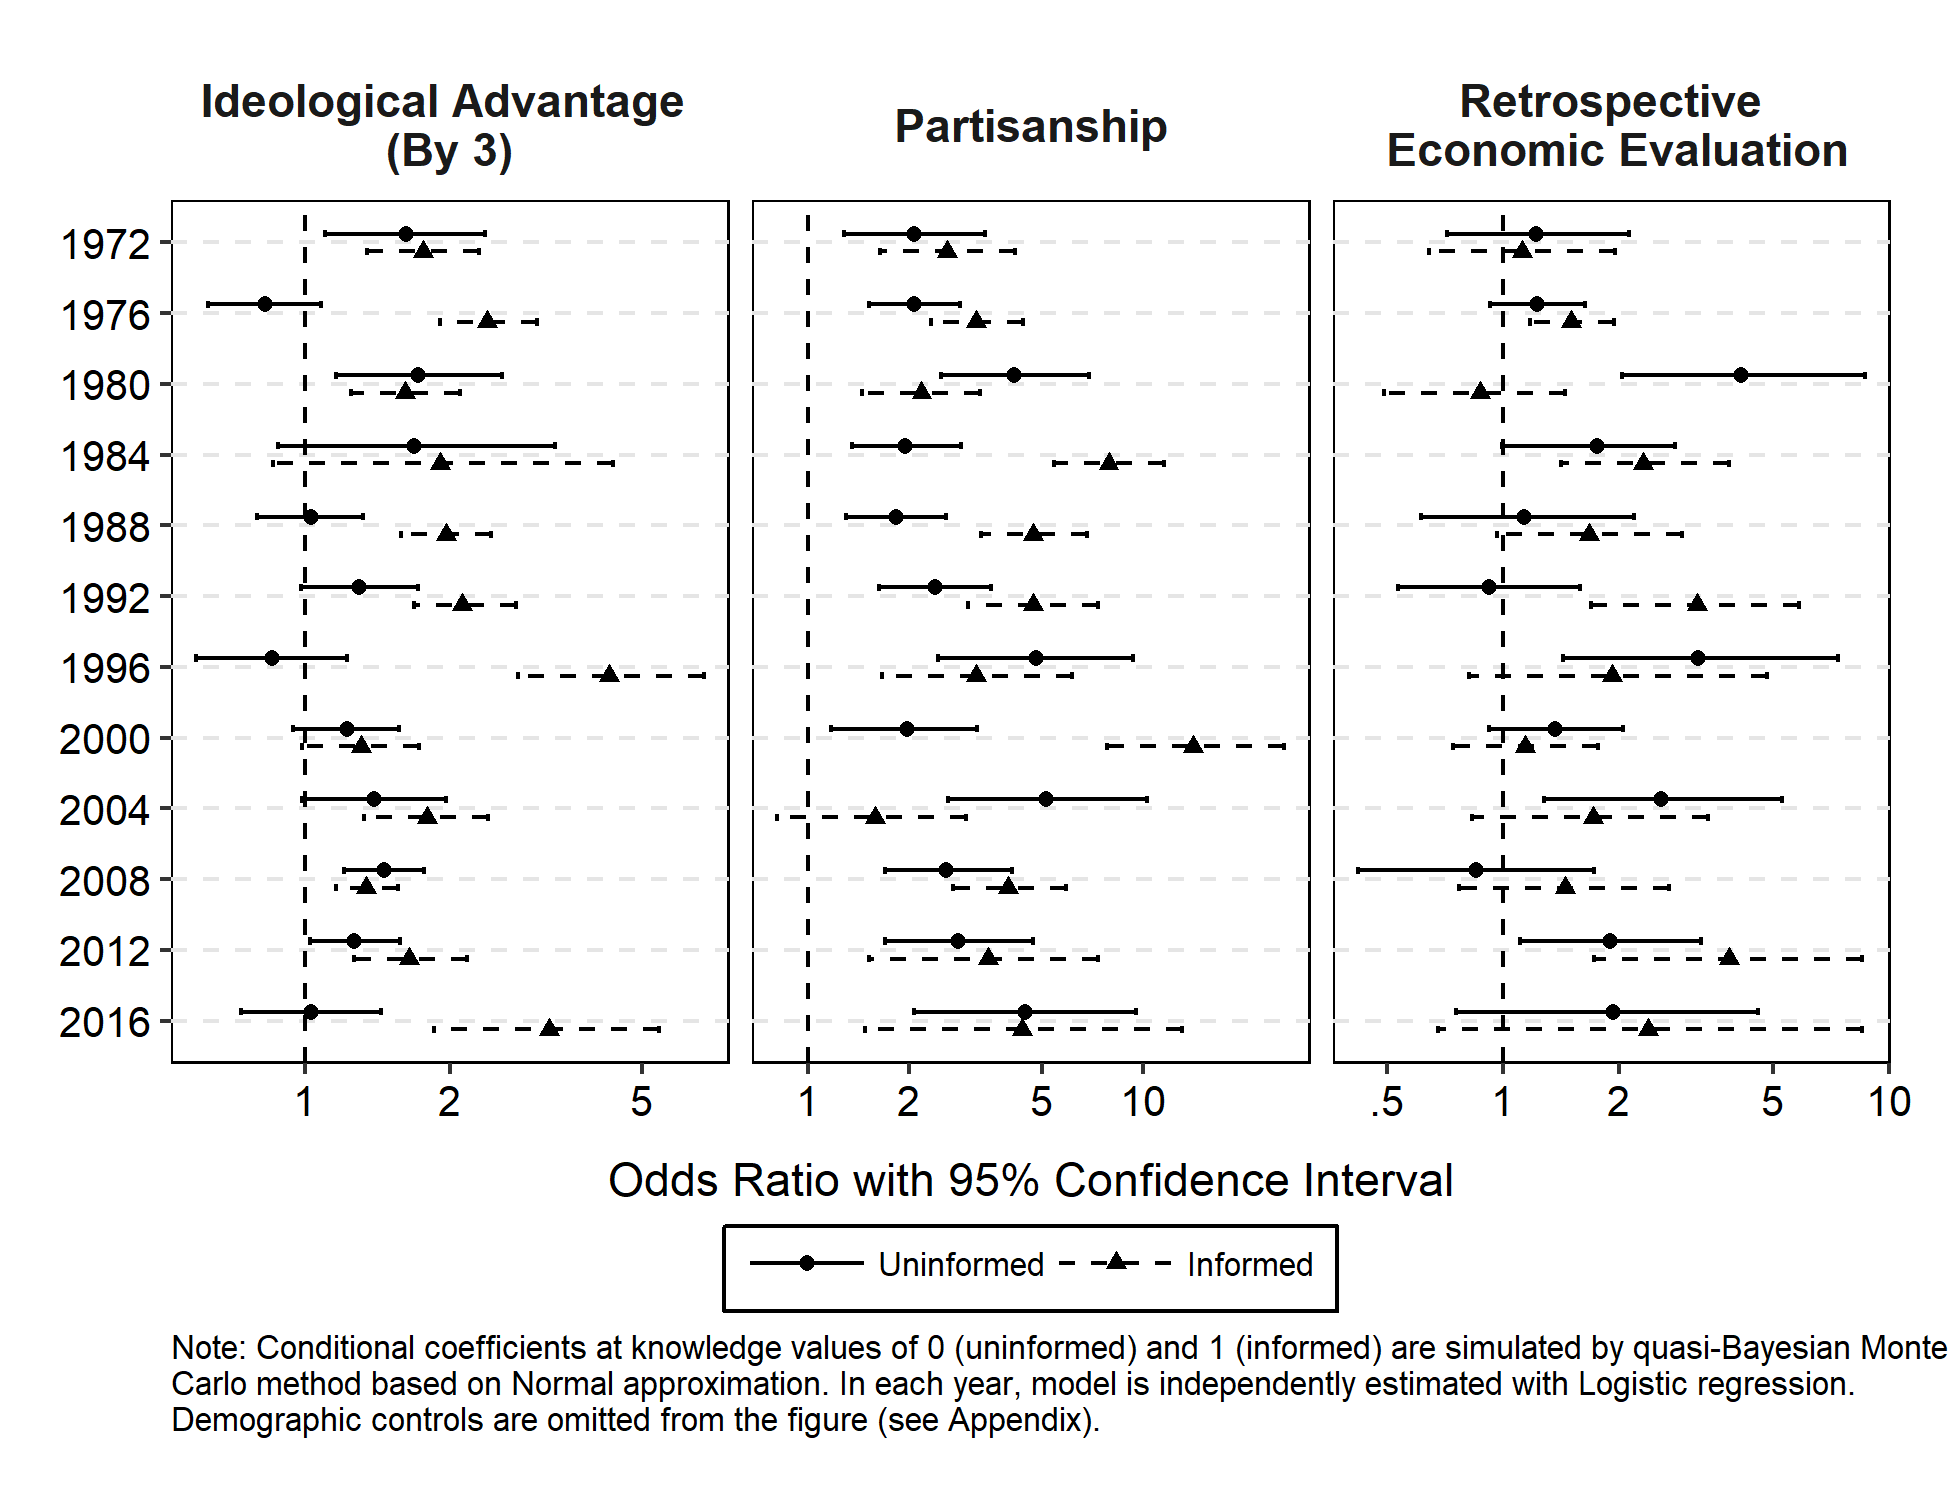
\includegraphics[width=\linewidth]{../outputs/m2sq_anescoefplot.png}
\end{figure}

\begin{figure}[ht!!!]
    \caption{The impact of demographic variables on presidential Vote Choice (1 = Republican, 0 = Democrat) in ANES Part I (1972-2016) (objective knowledge)}
    \label{fig:v2anescoefplot_dem1}
    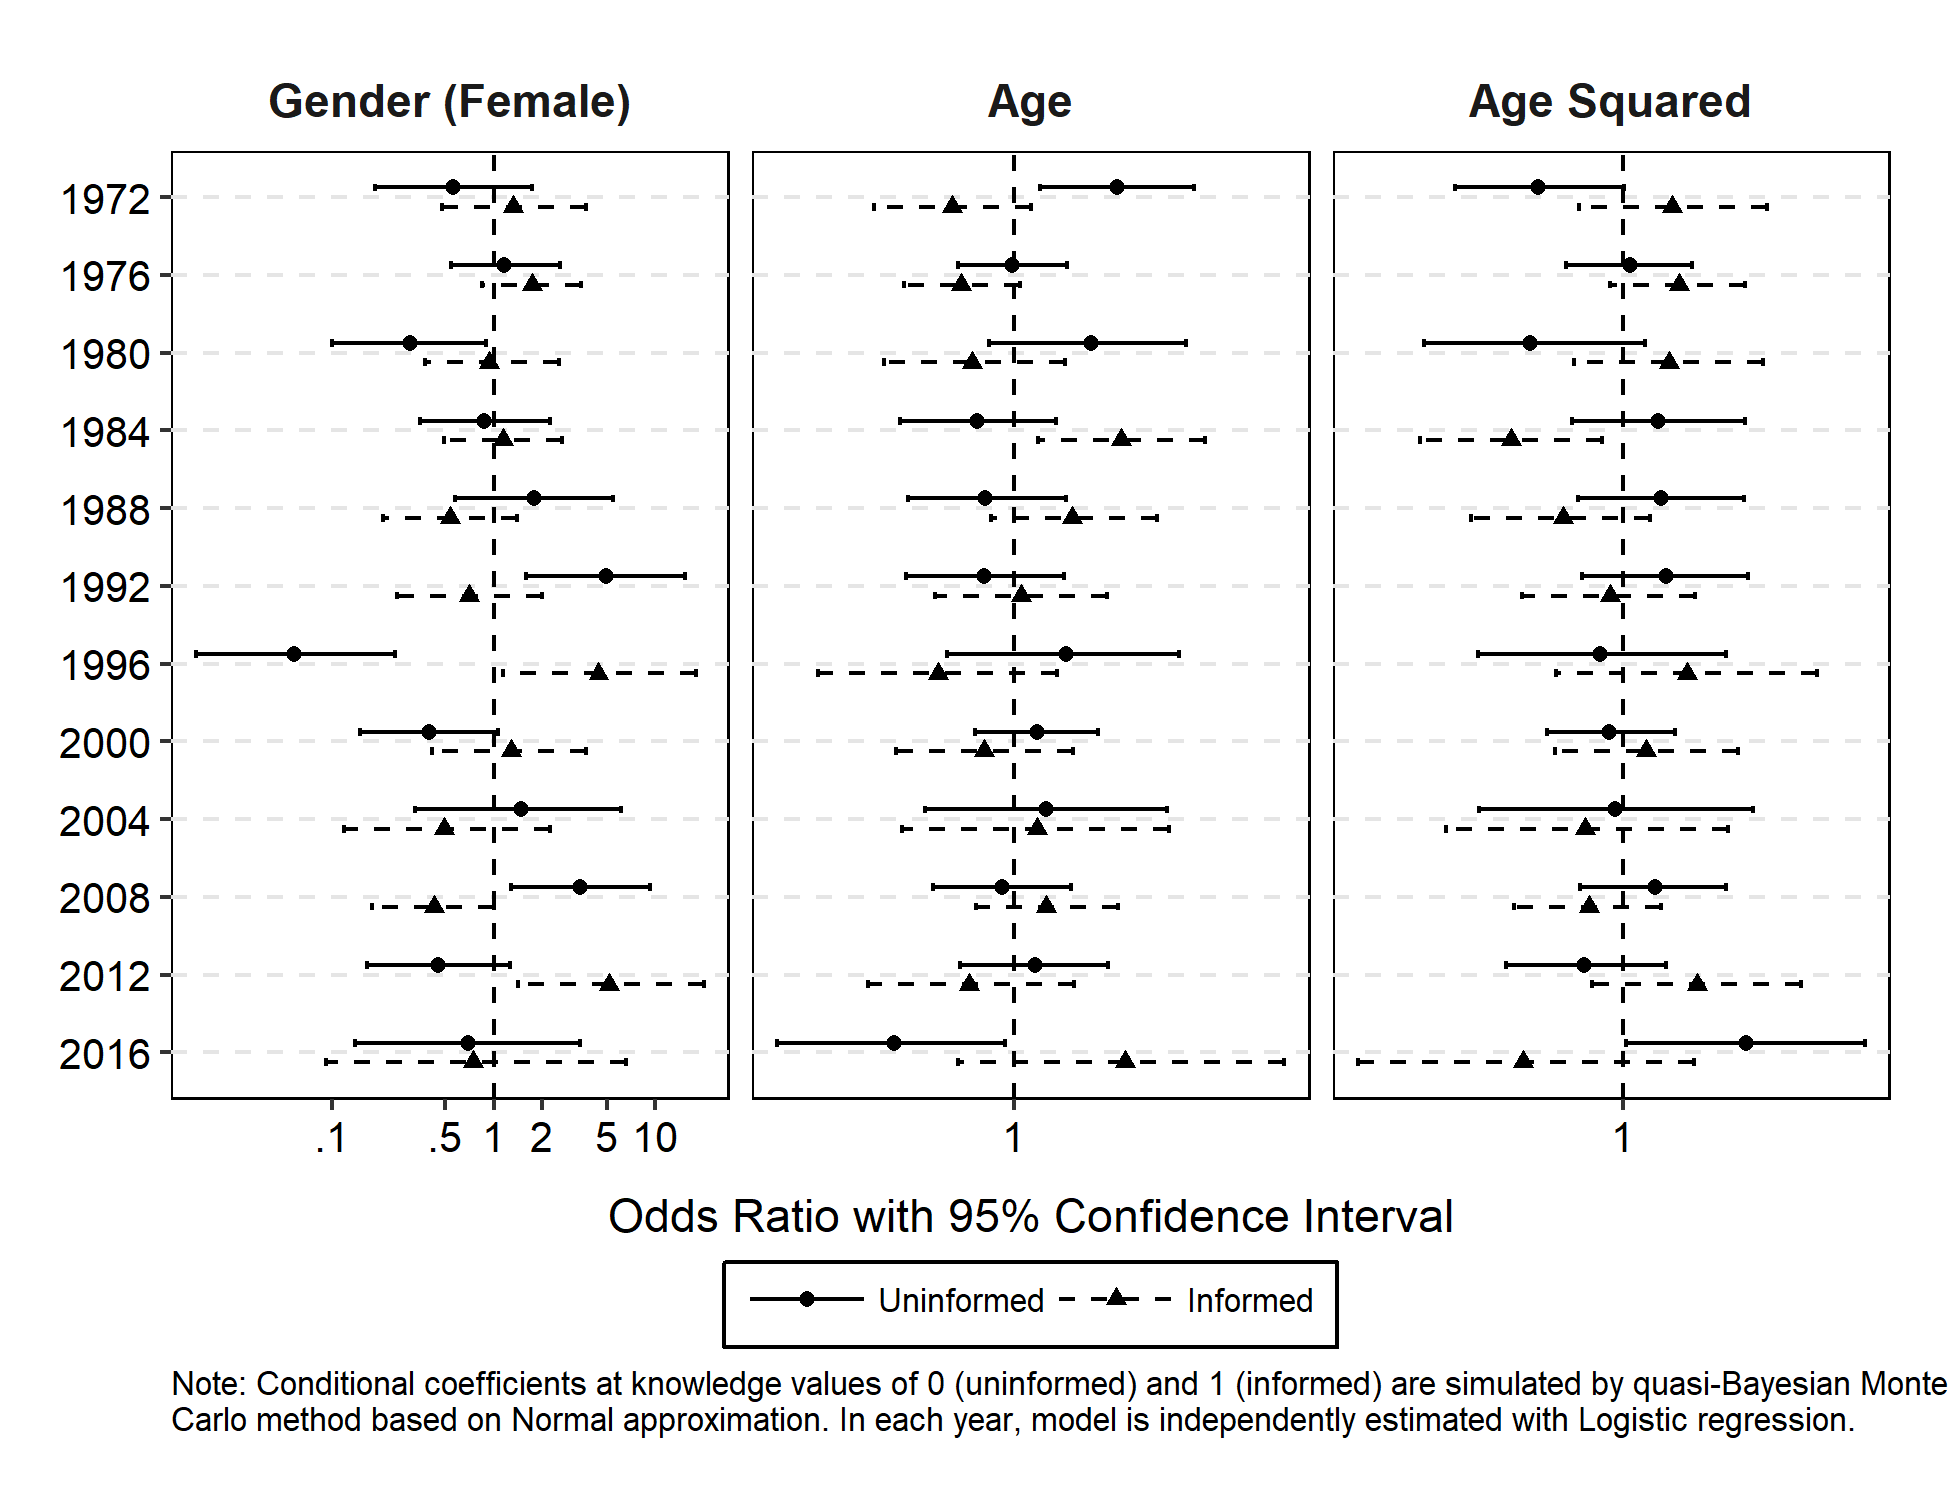
\includegraphics[width=\linewidth]{../outputs/m2sq_anescoefplot_dem1.png}
\end{figure}

\begin{figure}[ht!!!]
    \caption{The impact of demographic variables on presidential Vote Choice (1 = Republican, 0 = Democrat) in ANES Part II (1972-2016) (objective knowledge)}
    \label{fig:v2anescoefplot_dem2}
    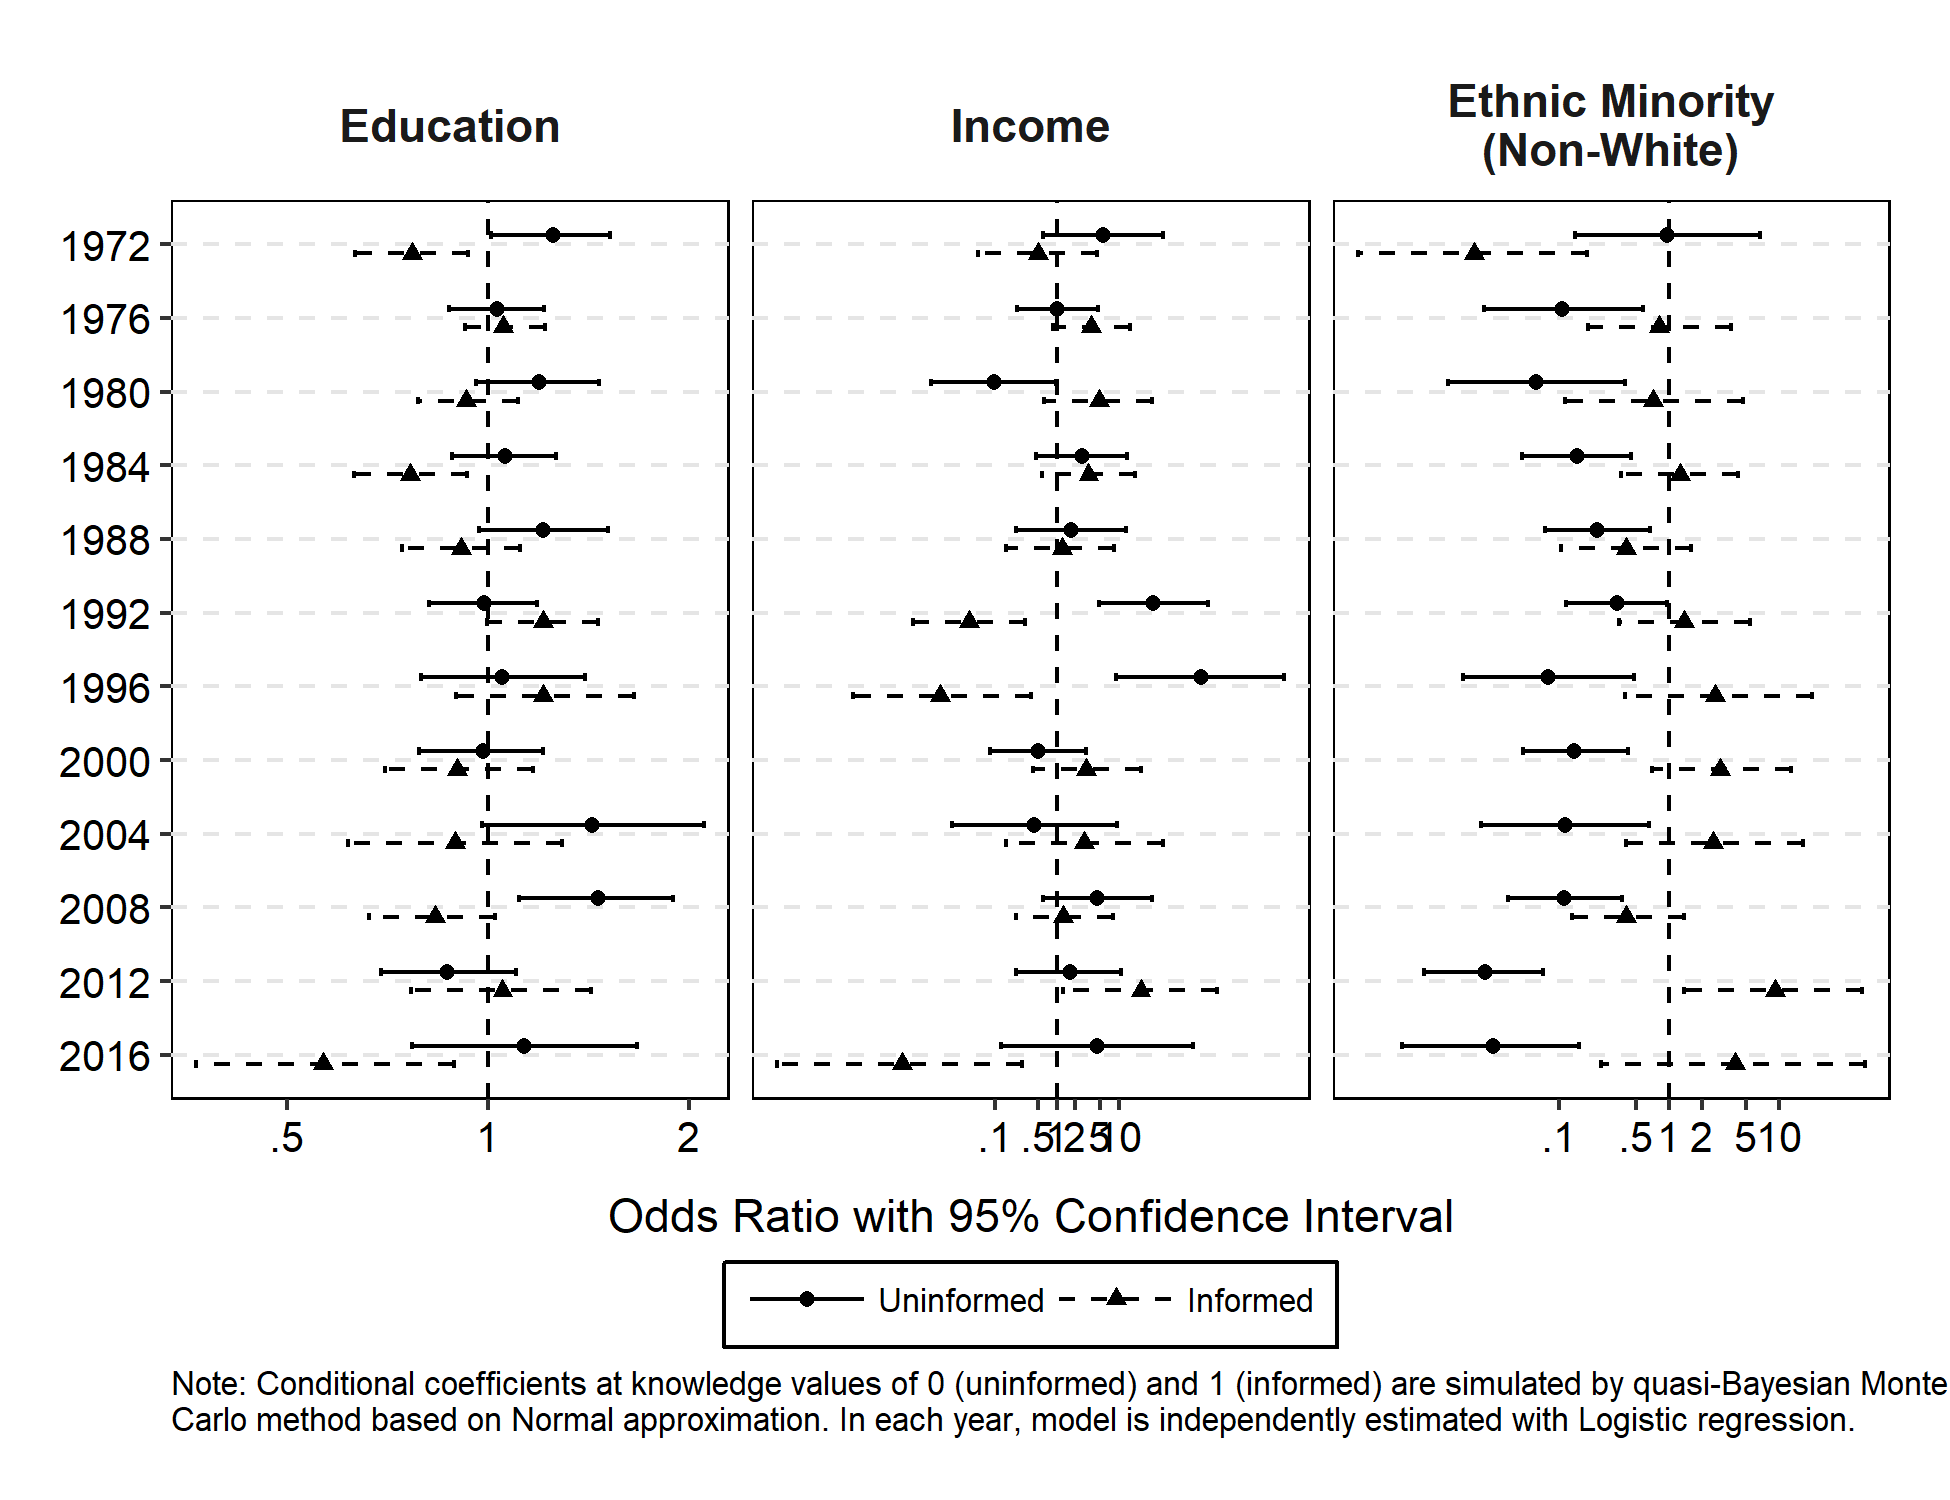
\includegraphics[width=\linewidth]{../outputs/m2sq_anescoefplot_dem2.png}
\end{figure}

\begin{figure}[ht!!!]
    \caption{The impact of demographic variables on presidential Vote Choice (1 = Republican, 0 = Democrat) in ANES Part III (1972-2016) (objective knowledge)}
    \label{fig:v2anescoefplot_dem3}
    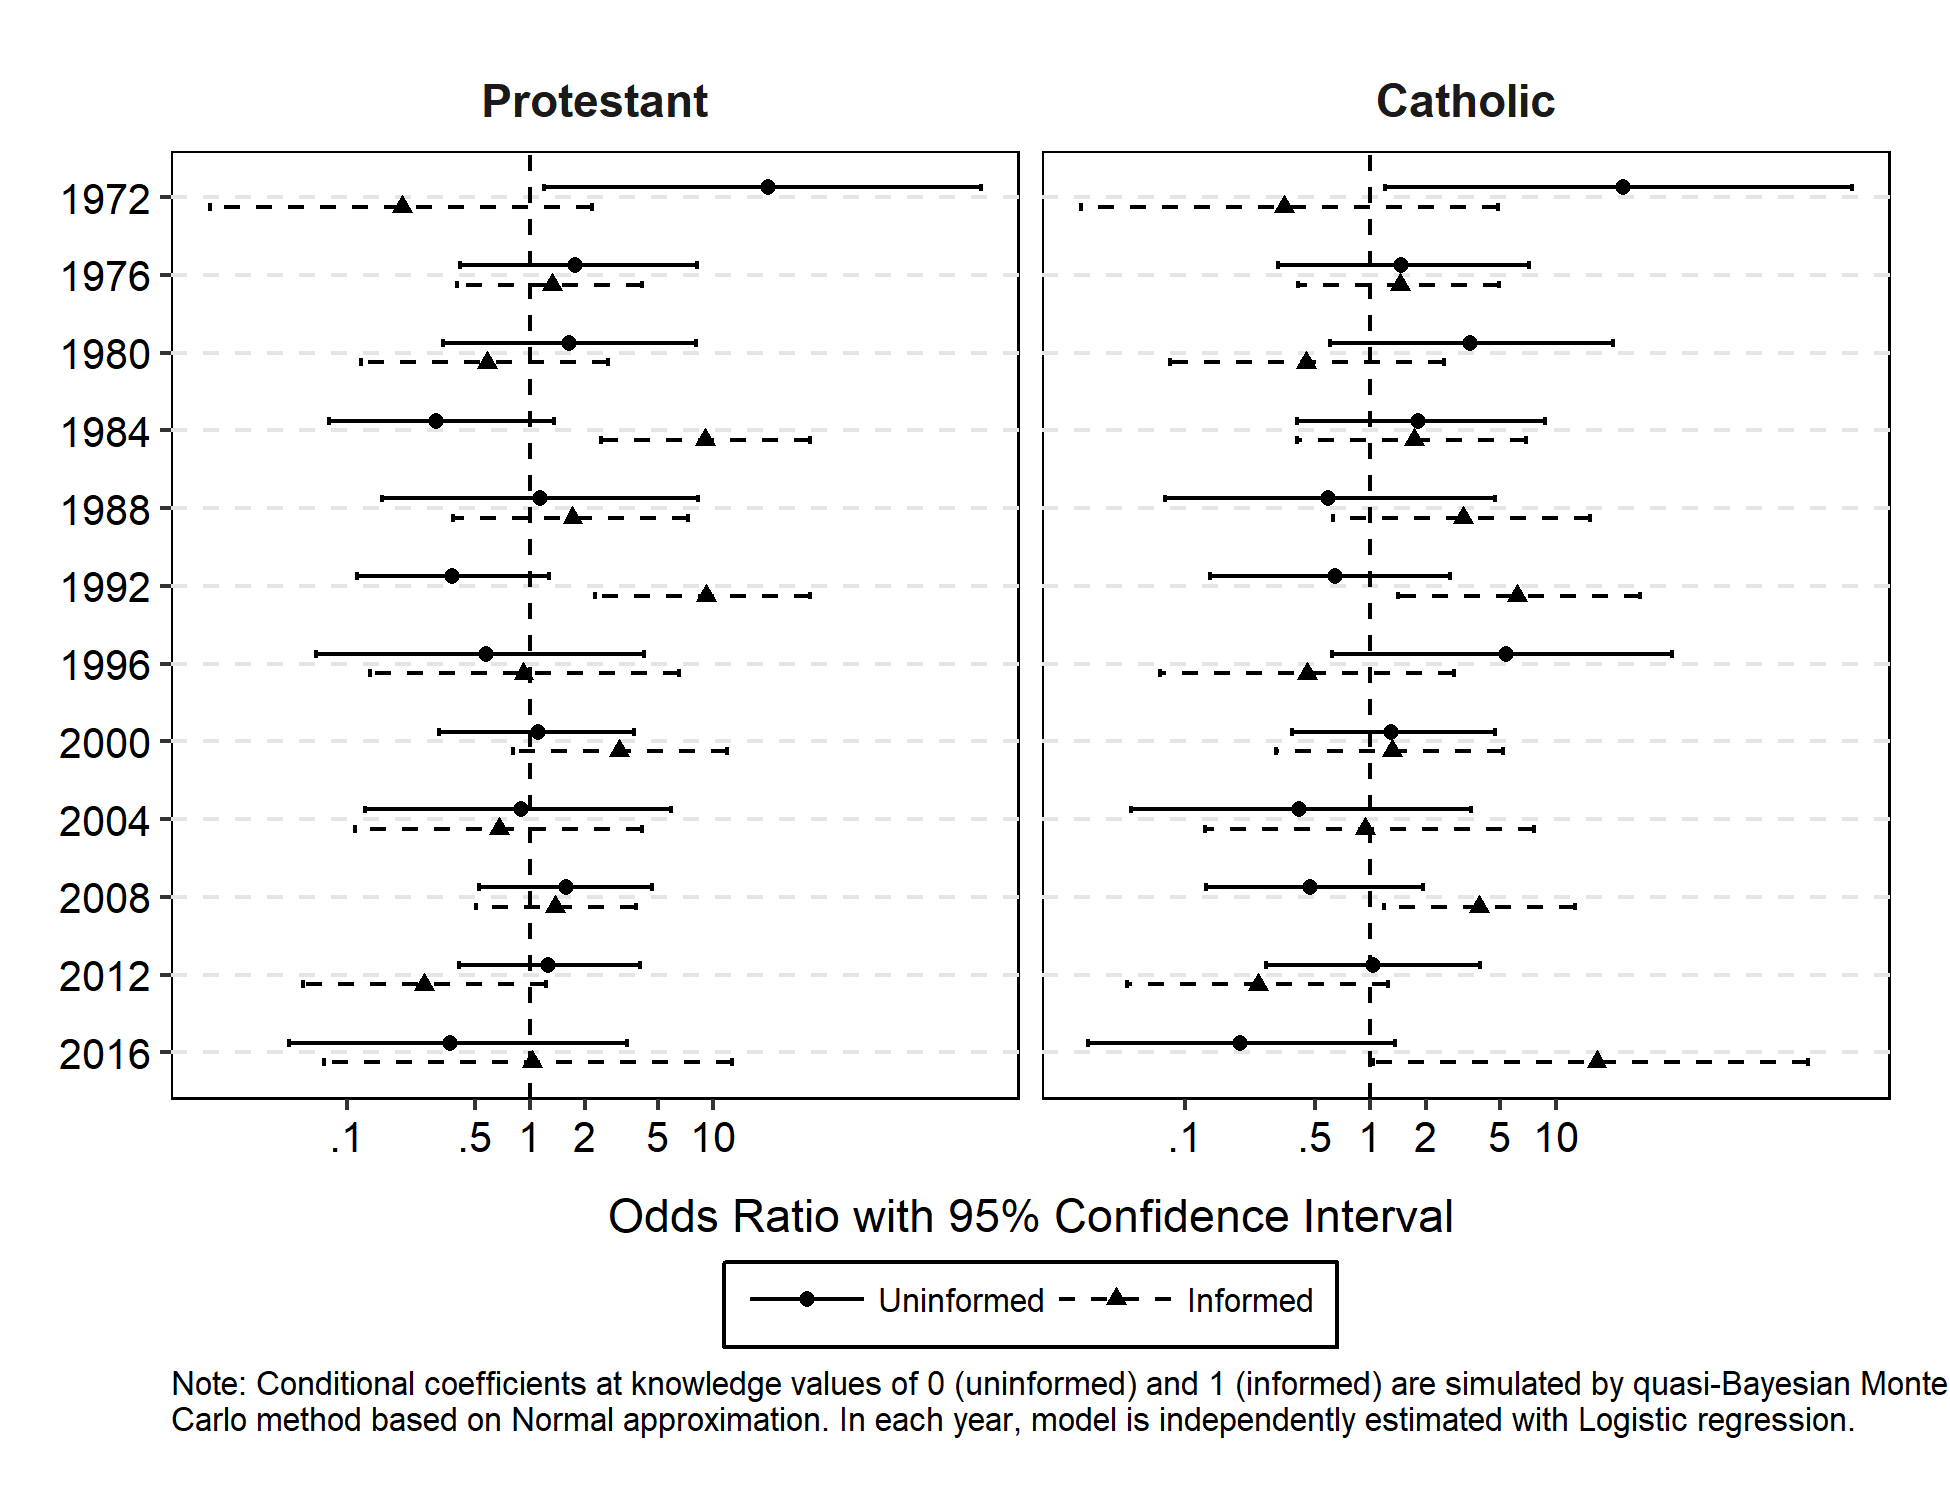
\includegraphics[width=\linewidth]{../outputs/m2sq_anescoefplot_dem3.png}
\end{figure}

\par In addition, \autoref{fig:v2anespredtable} shows the result comparable to \autoref{fig:anespredtable}, this time for objective knowledge. The result shows that the negative impact of national PVI on Republican vote choice persists (coefficient from EDV regression is statistically significant at 5\% level for all years but 2008). On the other hand, the effect of the incumbent party is weak and not statistically significant for most of the years.   

\begin{figure}[ht!!!]
    \caption{National partisan environment explains, but incumbent party does not explain predicted probability of Republican vote in ANES (1972-2016), estimated with voter profiles from different years (objective knowledge)}
    \label{fig:v2anespredtable}
    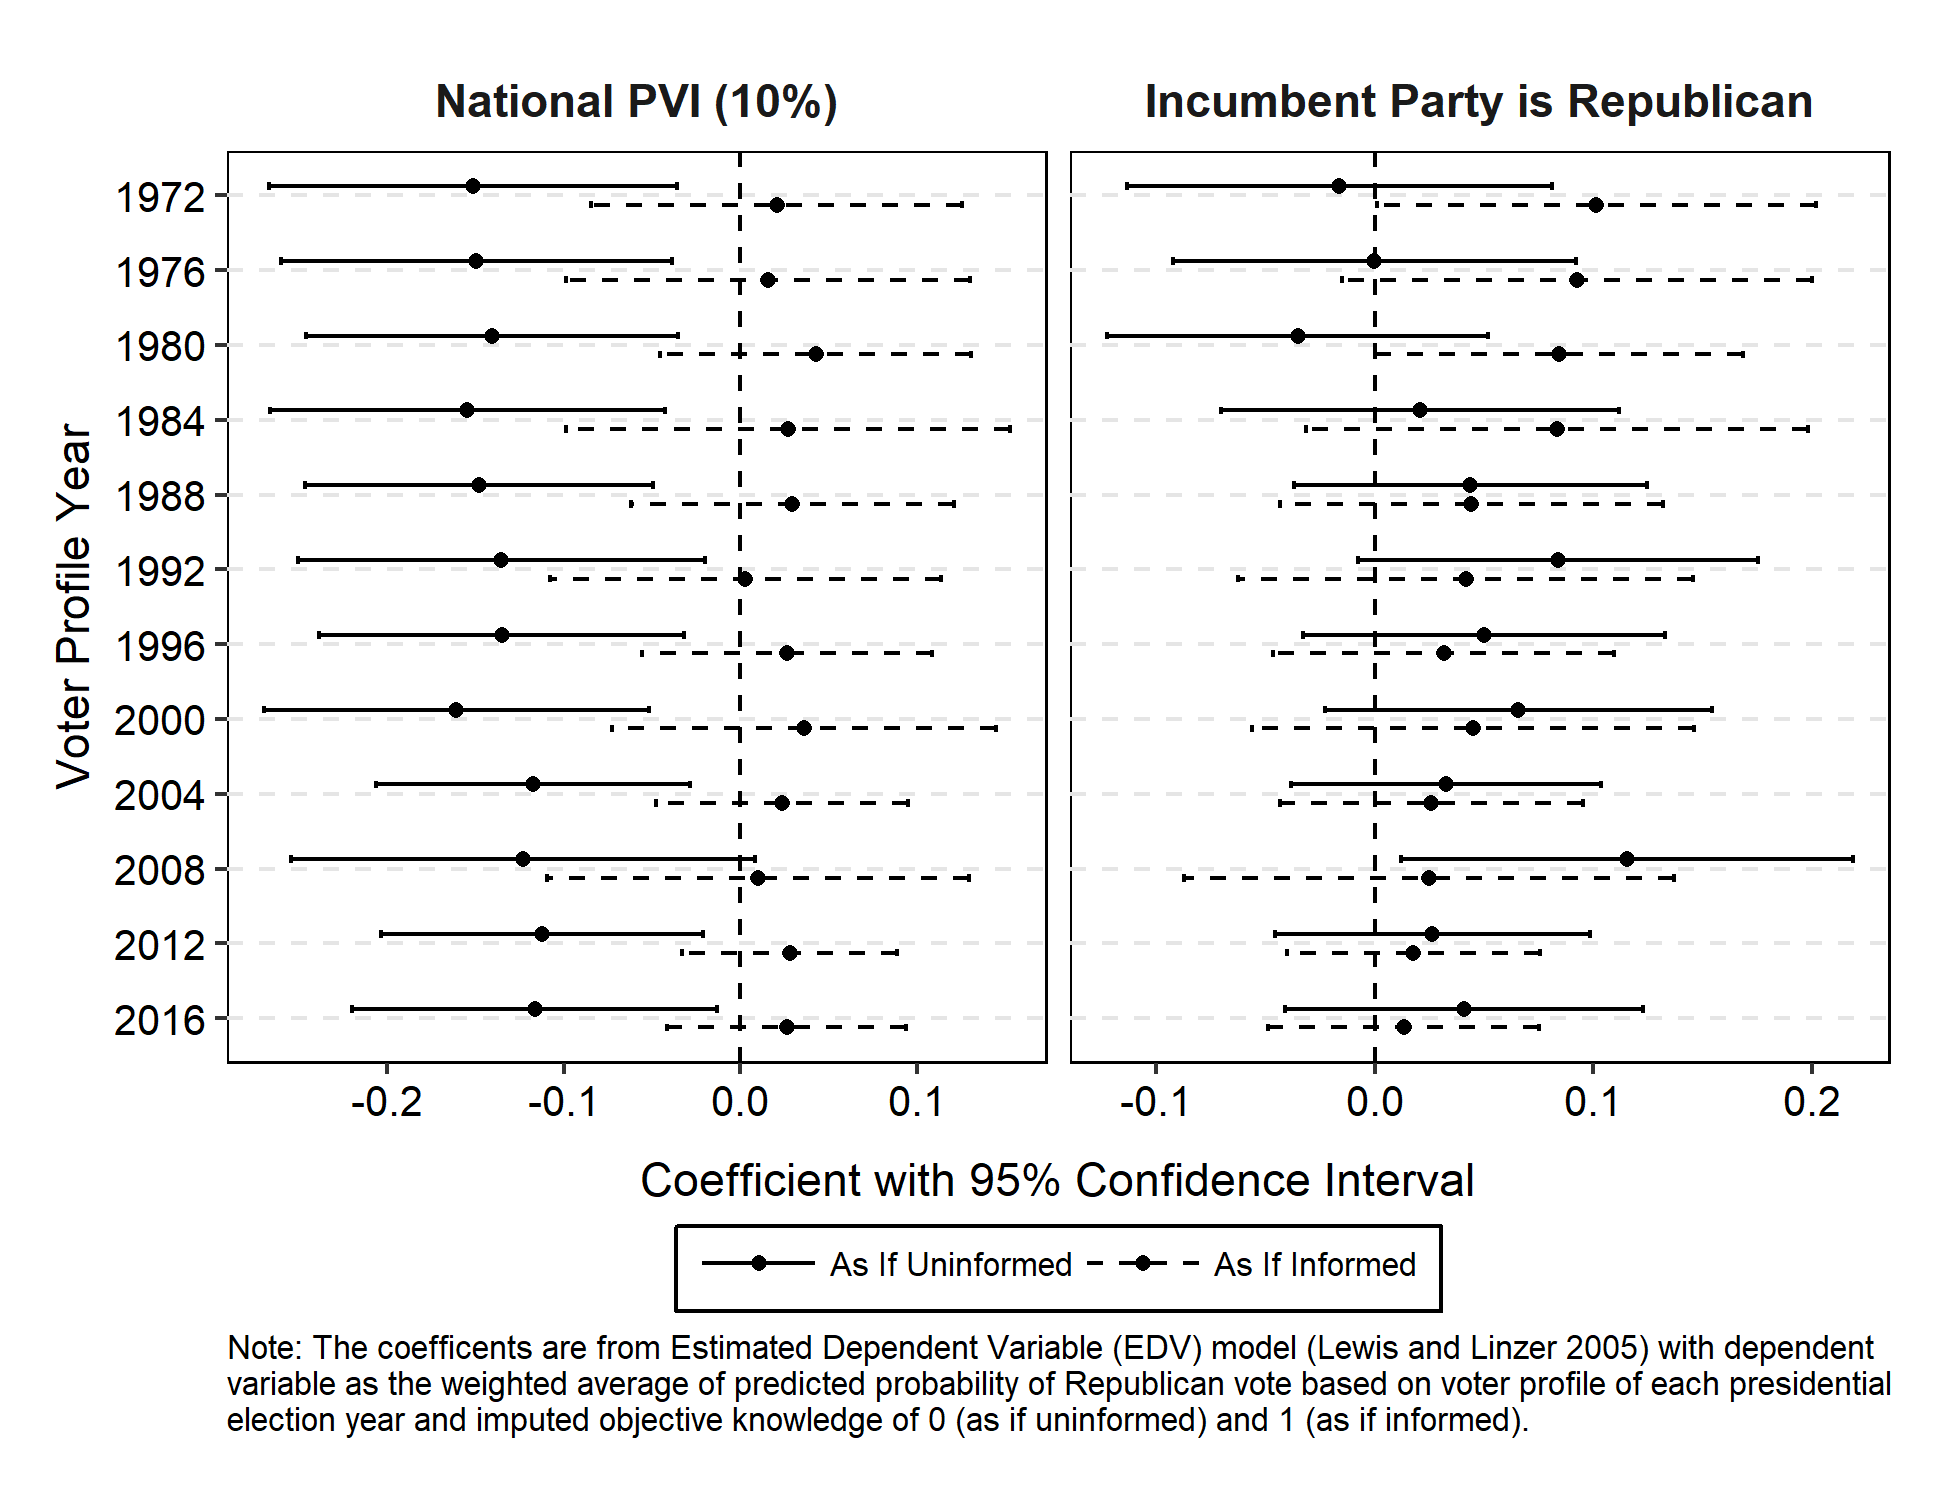
\includegraphics[width=\linewidth]{../outputs/m2sq_anespredtable.png}
\end{figure}

\clearpage
\section{Study 3 Appendix} \label{appC}
\setcounter{table}{0}
\renewcommand{\thetable}{C\arabic{table}}
\setcounter{figure}{0}
\renewcommand{\thefigure}{C\arabic{figure}}

\subsection{The Design of Agent-Based Simulation Model}

% latex table generated in R 3.5.1 by xtable 1.8-3 package
% Wed Jun 26 16:11:45 2019
\begin{table}[h!!!]
\centering
\caption{Voting Function Parameters} 
\label{voteparams}
\begin{tabular}{rrrrr}
  \hline
 & Mean & SE & lowerCI & upperCI \\ 
  \hline
Ideological Advantage & 0.198 & 0.044 & 0.125 & 0.269 \\ 
  Retrospective Evaluation & 0.716 & 0.251 & 0.306 & 1.129 \\ 
  Party Identity & 1.216 & 0.246 & 0.808 & 1.618 \\ 
  National PVI & -9.817 & 2.268 & -14.262 & -5.373 \\ 
  Incumbent (R) & 1.527 & 0.239 & 1.058 & 1.996 \\ 
  State PVI & 5.156 &  & 2.898 & 7.391 \\ 
  County PVI & 1.663 &  & 0.618 & 2.706 \\ 
   \hline
\end{tabular}
\end{table}


\par The voting function in the agent-based model is determined by the parameter values presented in \autoref{voteparams}. Focus on the Mean values of each parameter. First two rows describe the distribution of ANES individual preference coefficients for informed voters across 12 presidential elections occurred between 1972 and 2016. Those are used as coefficients for individual preferences in the PREFERENCE function. The third row represents the distribution of coefficients for party identity in ANES analysis, averaged across both informed and uninformed conditions. This is used as the coefficient of group membership on voting. The fourth and fifth row represents the distribution of ANES uninformed  coefficients for national PVI and Republican incumbent (using interviewer's rating of knowledge).\footnote{Since voting preference score is later converted to probability of voting by inverse logit function,  the EDV models are refitted to predict the average value of logit instead of the average predicted probability of Republican vote. The mean values presented are slightly different from the final value used in the ABM model (see main text), but this difference has no substantive impact on the results.}  Those are used as the coefficients for national PVI and incumbent advantage. Lastly, The sixth and seventh rows represent the CCES uninformed coefficients for state and county PVIs, averaged across 2008 and 2016. These are used as the coefficient for regional and sub-regional PVI in a voting function.      

% latex table generated in R 3.5.1 by xtable 1.8-3 package
% Wed Jun 26 16:11:45 2019
\begin{table}[h!!!]
\centering
\caption{Society Parameters} 
\label{socparams}
\begin{tabular}{rrrrr}
  \hline
 & Mean & SD & Lower 95\% CI & Upper 95\% CI \\ 
  \hline
Retrospective Evaluation (Mean) & -0.141 & 0.689 & -1.417 & 0.958 \\ 
  Rep. Ideology Perception (Mean) & 0.881 & 0.343 & 0.191 & 1.247 \\ 
  Dem. Ideology Perception (Mean) & -0.833 & 0.430 & -1.324 & -0.075 \\ 
  Ideology Distance from Rep. (SD) & 1.969 & 0.314 & 1.482 & 2.392 \\ 
  Ideology Distance from Dem. (SD) & 2.013 & 0.307 & 1.463 & 2.435 \\ 
  Self Ideology (Mean) & 0.282 & 0.129 & 0.087 & 0.466 \\ 
  Self Ideology (SD) & 1.374 & 0.157 & 1.161 & 1.596 \\ 
  Rep. Member Self Ideology (Mean) & 1.088 & 0.266 & 0.625 & 1.372 \\ 
  Rep. Member Self Ideology (SD) & 1.069 & 0.085 & 0.994 & 1.262 \\ 
  Dem. Member Self Ideology (Mean) & -0.397 & 0.267 & -0.904 & -0.120 \\ 
  Dem. Member Self Ideology (SD) & 1.245 & 0.101 & 1.109 & 1.405 \\ 
  Knowledge (Mean) & 0.638 & 0.047 & 0.593 & 0.714 \\ 
  Knowledge (SD) & 0.253 & 0.008 & 0.241 & 0.265 \\ 
   \hline
\end{tabular}
\end{table}


\par The fixed parameters of society are determined by the values presented in \autoref{socparams}. All data are obtained from ANES 1976-2016. To start with, the capacity of the incumbent party is drawn at each election from the normal distribution with mean 0 and standard deviation 0.5. This approximates the values presented in the first row. The observed mean of retrospective evaluation is -0.141, which is close enough to 0. The observed standard deviation is 0.689, but in the model, the value is reduced to 0.5, because higher than 0.5 standard deviation cause unrealistically large fluctuations in the voting behavior. 

\par The ideology of two parties are fixed at -0.8 (for blue) and 0.8 (for red). This value follows the mean values of ideology location perception given in the second and third rows of the table. Also, the mean of the common factor $\alpha$ in ideology function starts at 0 at the first election, given that the mean of self ideology over the years is close to 0 (6th row). The level of uncertainty in personal factor of ideology (i.e., the standard deviation of the normal distribution that generates $\epsilon_i$) is fixed at 1 given that observed average level of standard deviation in self-ideology within each survey (and within each party group) is close to 1 (7th, 9th, and 11th row). The effect of group membership on ideology $\beta$ is also fixed at 1, because the average value of ideology, especially among Republican party is close to 1 (i.e., which is consistent with model formulation $(\beta = 1) \times (g_i = 1) = 1$). It should be noted that the observed average value of ideology in Democratic party is smaller (i.e., -0.397) than what is set in the model (i.e., $(\beta = 1) \times (g_i = -1) = -1$). Furthermore, the average level of knowledge is fixed at 0.65, given the result at 12th row (interviewer's rating of knowledge). The model values are also manipulated to get the standard deviation of approximately 0.25 in the knowledge distribution of the society (referred to 13th row).   

\par Lastly, within each ANES survey, the ideological distance from Republican or Democratic candidates have the standard deviation of approximately 1.9 on average (fourth and fifth rows of the table). Therefore, given the fixed value of voter ideology, party position, and knowledge, the extent of signal-noise is manipulated so that the ideological distance measure yields the standard deviation of 1.9.     

\clearpage
\subsection{Comparison with Other Types of Context-based Uninformed Voting}

\par Figures below illustrates that use of both national-level balancing and local-level bandwagoning is the most effective way to make context-based uninformed decisions.

\begin{figure}[ht!!!]
    \caption{The loss in average utility under context-based, national-context-based, and local-context-based uninformed voting}
    \label{fig:abmres3c}
    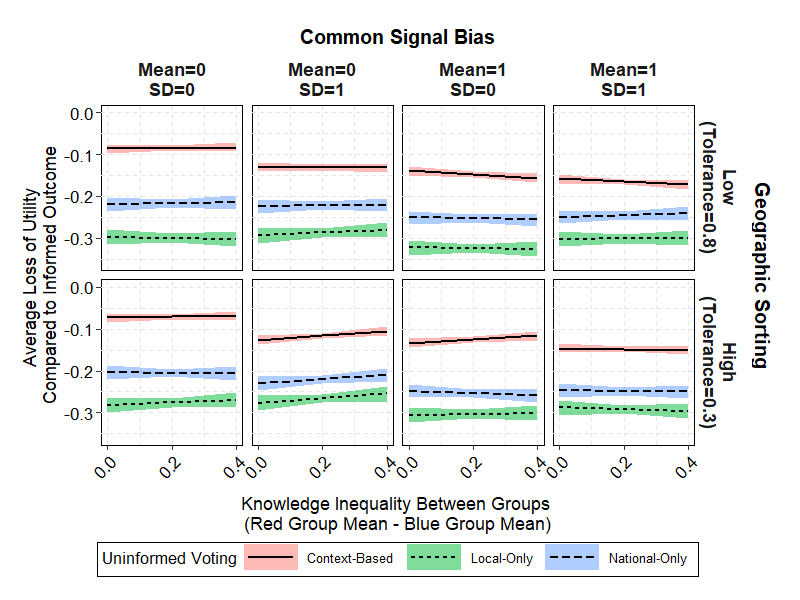
\includegraphics[width=\linewidth]{../outputs/abmres3c.png}
\end{figure}

\begin{figure}[ht!!!]
    \caption{The difference in average utility loss between blue and red voter groups under context-based, national-context-based, and local-context-based uninformed voting}
    \label{fig:abmres4c}
    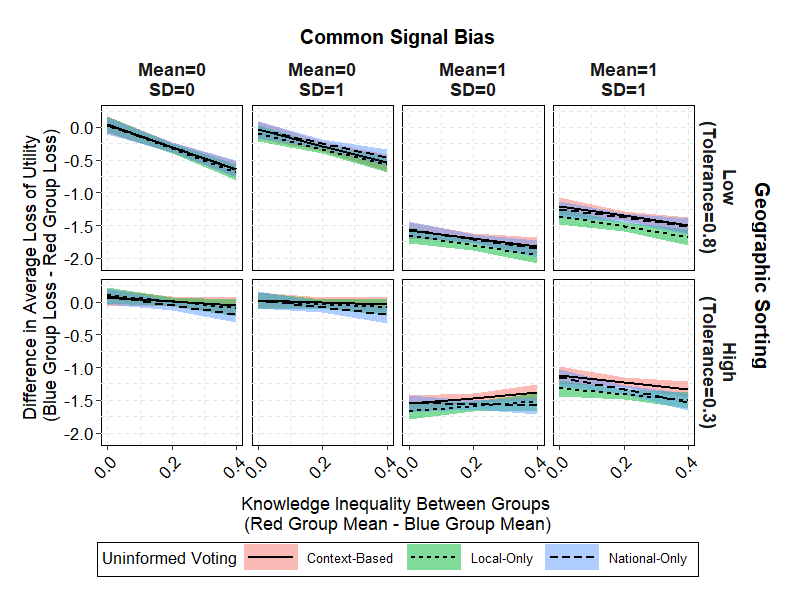
\includegraphics[width=\linewidth]{../outputs/abmres4c.png}
\end{figure}


\clearpage
\subsection{Additional Assessments of the Quality Electoral Outcome}

\par Following figures provide additional assessments of the quality of the democratic outcome. Two additional measures are considered here: (1) the average deviation in the vote share from informed outcomes, and (2) the probability of having the same winner as informed voters. Two measures give insights to the effectiveness of context-based uninformed voting similar to that of already presented measures. 

\begin{figure}[ht!!!]
    \caption{The average deviation in the vote share from the fully informed outcome under context-based and signal-based uninformed voting}
    \label{fig:abmres1}
    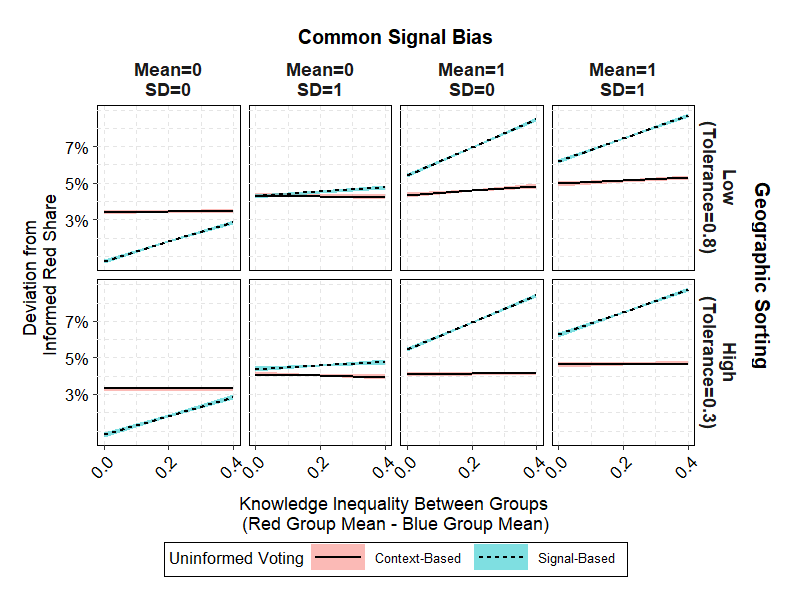
\includegraphics[width=\linewidth]{../outputs/abmres1.png}
\end{figure}

\begin{figure}[ht!!!]
    \caption{The average probability of having the same winner as the fully informed outcome under context-based and signal-based uninformed voting}
    \label{fig:abmres2}
    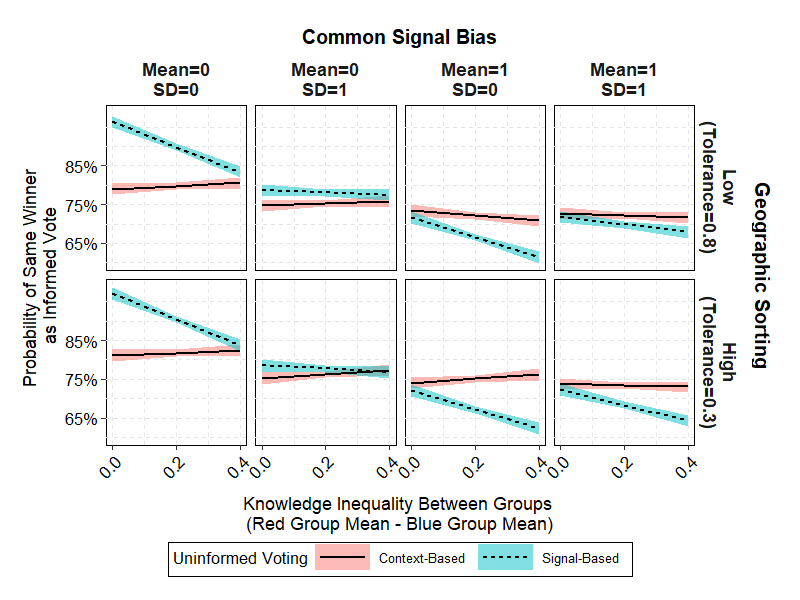
\includegraphics[width=\linewidth]{../outputs/abmres2.png}
\end{figure}

\begin{figure}[ht!!!]
    \caption{The average deviation in the vote share from the fully informed outcome under context-based, national-context-based, and local-context-based uninformed voting}
    \label{fig:abmres1c}
    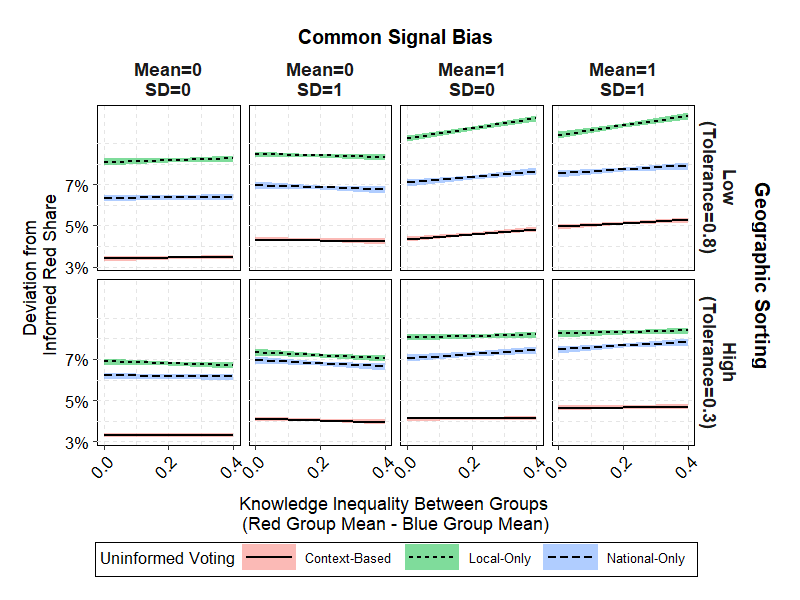
\includegraphics[width=\linewidth]{../outputs/abmres1c.png}
\end{figure}

\begin{figure}[ht!!!]
    \caption{The average probability of having the same winner as the fully informed outcome under context-based, national-context-based, and local-context-based uninformed voting}
    \label{fig:abmres2c}
    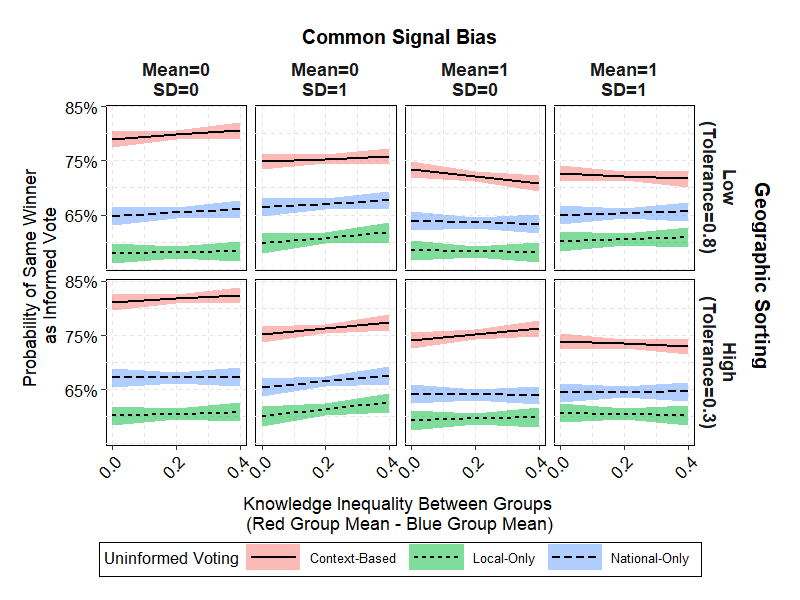
\includegraphics[width=\linewidth]{../outputs/abmres2c.png}
\end{figure}


